\documentclass[conference, compsocconf]{IEEEtran}
\IEEEoverridecommandlockouts

\usepackage{xcolor}
\usepackage{url}
\usepackage{rotating}
\usepackage{subfig}
\usepackage{listings}
\usepackage{amsthm}
\usepackage[linesnumbered,boxed,ruled,nofillcomment]{algorithm2e}
\usepackage{booktabs}

\lstset{frame=lines,escapeinside={(*@}{@*)},language=Java,captionpos=b,tabsize=3,numbers=left,numberstyle=\tiny,numbersep=5pt,breaklines=true,showstringspaces=false,basicstyle=\scriptsize,emph={label}}


% correct bad hyphenation here
\hyphenation{}


% Macros

\newcommand{\ie}{\textit{i.e.,} }
\newcommand{\eg}{\textit{e.g.,} }
\newcommand{\mukul}[1]{{\color{darkred}{\bf(**MP: #1**)}}}
\newcommand{\razieh}[1]{{\color{magenta}{\bf(**RNZ: #1**)}}}
\newcommand{\sarfraz}[1]{{\color{blue}{\bf(**SK: #1**)}}}

\def\denseitems{
  \itemsep1pt plus1pt minus1pt
  \parsep0pt plus0pt
  \parskip0pt
  \topsep0pt
}

\definecolor{darkred}{rgb}{0.75,0,0}
\newcommand{\remark}[1]{\textcolor{darkred}{\textbf{$\{$#1$\}$}}}
\newcommand{\todo}[1]{\textbf{\color{darkred} \textsc{ToDo:} #1}}
\newcommand{\tbd}{\textbf{\color{darkred} TBD.}}
\newcommand{\tool}{\textsc{Quantum}}
\newcommand{\NumApps}{\textsc{6}}
\newcommand{\NumBugs}{\textsc{22}}
\newcommand{\NumTests}{\textsc{60}}
\newcommand{\NumAppsStudy}{\textsc{13}}
\newcommand{\NumBugsStudy}{\textsc{106}}
\newtheorem{mydef}{Definition}

\newcommand{\Caption}[1]{\vspace*{-1ex}\caption{#1}\vspace*{-2ex}}
\newcommand{\Section}[1]{\vspace*{-1ex}\section{#1}\vspace*{-1ex}}
\newcommand{\Subsection}[1]{\vspace*{-1ex}\subsection{#1}\vspace*{-1ex}}

%\newcommand{\subparagraph}{}
%\usepackage[compact]{titlesec}
%\titlespacing{\section}{0pt}{1ex}{1ex}
%\titlespacing{\subsection}{0pt}{1ex}{0ex}
%\titlespacing{\subsubsection}{0pt}{0.5ex}{0ex}

\addtolength{\textfloatsep}{-0.2in}

% To reduce inter-line spacing
%\renewcommand{\baselinestretch}{0.93}
%\normalsize



\begin{document}
\title{Automated Generation of Oracles for Testing User-interaction Features of Mobile Apps}

\author{\IEEEauthorblockN{Razieh Nokhbeh Zaeem\IEEEauthorrefmark{1}\thanks{\IEEEauthorrefmark{1}
      This author was an Intern at Fujitsu Labs of America
      for a part of this work.}}
\IEEEauthorblockA{The University of Texas at Austin\\
%Austin, Texas 78712\\
nokhbeh@utexas.edu}
\and
\IEEEauthorblockN{Mukul R. Prasad}
\IEEEauthorblockA{Fujitsu Laboratories of America\\
%Sunnyvale, CA 94085\\
mukul@us.fujitsu.com}
\and
\IEEEauthorblockN{Sarfraz Khurshid}
\IEEEauthorblockA{The University of Texas at Austin\\
%Austin, Texas 78712\\
khurshid@ece.utexas.edu}
}

\maketitle


\begin{abstract}

As the use of mobile devices becomes increasingly ubiquitous, the need
for systematically testing applications (apps) that run on these
devices grows more and more.  However, testing mobile apps is
particularly expensive and tedious, often requiring substantial manual
effort.  While researchers have made much progress in automated
testing of mobile apps during recent years, a key problem that remains
largely untackled is the classic \emph{oracle} problem, i.e., to
determine the correctness of test executions.  This paper presents a
novel approach to automatically generate test cases, that include test oracles,
for mobile apps.
The foundation for our approach is a comprehensive study that we conducted of real defects in mobile
apps. Our key insight, from this study, is that
there is a class of features that we term \emph{user-interaction} features,
which is implicated in a significant fraction of bugs and for
which oracles can be constructed -- in an application agnostic manner --
based on our common understanding of how apps behave.  We present an extensible
framework that supports such domain specific, yet application
agnostic, test oracles, and allows generation of test sequences that
leverage these oracles.
Our tool, \tool, embodies our approach for generating test
cases that include oracles.  Experimental results using $\NumApps$ Android
apps show the effectiveness of \tool{} in finding potentially serious
bugs, while generating compact test suites for user-interaction features.

\end{abstract}

\IEEEpeerreviewmaketitle

\Section{Introduction}
\label{introduction}

% The rise and importance of mobile applications & the case for automated testing of mobile software
Recent years have witnessed an explosive growth in the use of mobile devices and in the number and variety of software applications developed for such devices. Mobile applications, or apps as they are popularly called, are often developed in small, fast-paced projects with scarce testing resources. At the same time, testing mobile apps presents some unique challenges, such as supporting a wide range of devices, platforms and versions, as well as ensuring the integrity of the rich and highly interactive user-interface characteristic of such apps~\cite{MobileDev:IBMWhitePaper}. Thus, there is a growing need to develop automated testing tools to support the development of mobile apps.

% Typically automated testing = test sequence generation
Researchers have made significant progress in developing techniques to support automated testing of mobile apps~\cite{Nguyen:2012:ISSTA, AnandFSE2012, AmalfitanoASE2012, Joorabchi:2012:WCRE, collider2013}. However, these techniques primarily target the generation of test sequences, leaving the task of adding test oracles~\cite{Oracle:Howden78, Weyuker80} into these test sequences to the human tester. This itself can be a manually intensive process and if the oracles are not of a sufficiently high quality, can potentially compromise the efficacy of test cases.

% Our aim & the bug-study
The aim of this paper is to partially address the oracle problem in the context of automated test case generation for mobile applications. To realize this aim we conducted a study where we sampled, studied and categorized the bugs reported for several popular, open-source Android applications. The study revealed that a significant fraction of bugs can be attributed to \emph{user-interaction} features that are supported by the mobile platform and simply implemented by each application. Such features include content presentation or navigation features such as rotating the device or using various gestures to scroll or zoom into screens. A distinguishing characteristic of these features is that they are largely independent of the core logic of the application. More importantly, there is often a general, common sense expectation of how the application should respond to a given feature. For example, rotating a device and then rotating it back should bring the display precisely back to the initial screen. Such observations motivate our approach.

% Summary of our approach
We present a novel framework for authoring test oracles for checking
user-interaction features of mobile applications, in an application
agnostic manner.  Our framework supports
\emph{model-driven test suite generation}~\cite{SwTestBk:2007} where each
generated test includes both the test sequence to execute and the
corresponding assertions to check (as test oracles).  Given 
a model of the user-interface of the mobile app under test, our
framework uses its built-in, extensible library of oracles (for
various user-interaction features) and generates a test suite to
comprehensively test the app against user-interaction
features.

While the basic goal of our framework is to allow generation of test
suites that are complete with embedded test oracles for supported
features, it includes two more techniques to further enhance its
usefulness in practice.  %Specifically, 
Firstly, our framework supports a customizable \emph{cost} 
function that defines a measure of cost for executing %a transition in the input model 
a given test suite and produces an output suite that has likely minimal 
execution cost, while checking each feature.
Secondly, our test generation technique inserts multiple test oracles, for 
\emph{different} features, within a \emph{single} test case, when possible.
This allows checking of multiple properties within the same test execution,
by conceptually sharing execution segments common across different tests,
thus reducing the overall test execution cost.
% and reducing the total overhead of executing test suites for mobile apps, which
%typically require high execution overhead due to their event-driven functionality.  
Our test generation technique produces
\emph{feature-adequate} test suites, which for the given
model exercise every transition relevant to each supported feature and
test its expected functionality.

% A few sentences about our tool and results
Our tool, \tool, embodies our framework and provides a fully
automated, \emph{push-button} tool-set for test case generation for
mobile apps.  Our initial experiments with \tool{} show that it generates
valuable test suites and provides the foundation of a promising
approach for more effective testing of mobile apps.

% Main Contributions
This paper makes the following contributions:

%\begin{itemize}\denseitems

%\item
{\bf Bug study}.  We perform a comprehensive study of
          real mobile application defects and identify a family of
          mobile application features, which we term \textit{user-interaction features}. We observe that these features are 
          implicated in a significant fraction of the studied defects. 
          Further, they are characteristic of the mobile platform and implemented 
          by many mobile applications but not directly dependent on the
          application logic.          
\\
%\item
\indent{\bf Feature-driven testing of mobile apps}.   We introduce a novel form of
          \emph{test adequacy}~\cite{GoodenoughGerhart1975} in the context of mobile apps where the
          goal is to cover the given model of the app's user-interface
          by exercising each transition relevant to any desired
          feature and checking the expected functionality for the feature.
\\
%\item 
\indent{\bf Automatic oracle generation for testing mobile apps}. We present an extensible 
				  library of oracles for various user-interaction features.
				  % along with how to use those features to automatically generate test oracles. 
				  Our framework allows authoring test oracles for features, in an
	        application agnostic manner, for re-use across a number of
	        different apps that are expected to support those features.   
	        These oracles are appropriately instantiated by our model-driven
	        test suite generation technique. 
\\
%\item 
\indent{\bf Minimal cost test suite generation}. We provide a technique for generating a
          compact test suite by trying to minimize a customizable cost function. 
          The test suite also incorporates the oracles to comprehensively test the supported feature set.
\\
%\item 
\indent{\bf Evaluation}.  We present our tool, \tool{}, for
          automated testing of mobile apps and its evaluation on
          $\NumApps$ real Android applications.  The evaluation
          confirms that \tool{} is able to generate compact
          test suites, complete with test oracles, for testing the
          identified features. These test suites are able to reveal
          a number of bugs in the studied
          applications: \tool{} found a total of $\NumBugs$ bugs, 
          a few of them particularly serious, using a total of $\NumTests$ tests for these $\NumApps$ apps.
%\end{itemize}

\section{Bug Study}
\label{study}


%Despite all the progress made to automate testing, mobile apps still suffer from a range of bugs. The presence of bugs, in addition to inherent differences between mobile apps and traditional programs, motivated us to study the nature of bugs in mobile apps to develop more targeted and customized automated testing strategies for them. 
We conducted a bug study on $\NumBugsStudy$ bugs drawn from $\NumAppsStudy$ open-source Android applications. The aim was to identify opportunities for automatically generating test cases, that include test oracles, by focusing on bugs specific to mobile apps and by exploiting domain knowledge of the mobile platform.
%Using this study, we identified several challenging aspects of mobile apps, with a focus on open-source Android apps, in order to craft a customized testing strategy that suits mobile apps and more effectively finds bugs in them.

The $\NumAppsStudy$ open-source Android apps we selected %mostly form Google Code\footnote{https://code.google.com}. 
included $6$ apps studied in previously published work on automated testing for mobile apps~\cite{Hu:2011:AST,AmalfitanoASE2012,Nguyen:2012:ISSTA}, a further $6$ apps selected from the open source repository Google Code, and the \textit{Notepad} sample app provided for educational purposes by the official Android website (also studied in previous work~\cite{Nguyen:2012:ISSTA}). Table~\ref{tab:studySubjects} lists the name, stated function, and source for each of the $\NumAppsStudy$ subjects.

\begin{table}
\caption{Subjects for Bug Study.}
\label{tab:studySubjects}
\begin{center}
\begin{tabular}{lll}
\toprule
\textbf{App} & \textbf{Function} & \textbf{Source} \\
\midrule
\textit{Notepad} &  Note Making Tool & \url{developer.android.com/tools/samples}\\
\textit{CMIS} & CMIS Browser & \url{gc/android-cmis-browser} \\
\textit{Delicious} & Social Bookmarking & \url{gc/android-delicious-bookmarks} \\
\textit{OpenSudoku} & Sudoku Game & \url{gc/opensudoku-android} \\
\textit{MonolithAndroid} & 3D Game & \url{gc/monolithandroid} \\
\textit{Wordpress} & Blogging Tool & \url{android.trac.wordpress.org} \\
\textit{Nexes Manager} & File Manager & \url{github.com/nexes/Android-File-Manager} \\
\midrule
\textit{VuDroid} & PDF Viewer & \url{gc/vudroid} \\
\textit{Kitchen Timer} & Timer & \url{gc/kitchentimer} \\
\textit{Dolphin Player} & Media Player & \url{gc/dolphin-player} \\
\textit{AnkiDroid} & Flashcard Review & \url{gc/ankidroid} \\
\textit{Shuffle} & Personal Organizer & \url{gc/android-shuffle} \\
\textit{K9Mail} & Email Client & \url{gc/k9mail} \\
\bottomrule
\end{tabular}
\end{center}
gc: \url{https://code.google.com/p}
\end{table}

%To minimize threats to validity, we first considered apps studied in previous published work~\cite{Hu:2011:AST,AmalfitanoASE2012,Nguyen:2012:ISSTA}: CMIS\footnote{https://code.google.com/p/android-cmis-browser} is a CMIS browser, Android Delicious\footnote{https://code.google.com/p/android-delicious-bookmarks} is a social bookmarking application, OpenSudoku\footnote{https://code.google.com/p/opensudoku-android} is a Sudoku game, MonolithAndroid\footnote{https://code.google.com/p/monolithandroid} (renamed to Robotic Space Rock) is a 3D game, WordPress\footnote{http://android.trac.wordpress.org} is a blogging tool, and K9Mail\footnote{https://code.google.com/p/k9mail} is an email client. 

%% Test Subject Selection
Our aim was to choose test subjects from a diverse set of application categories and functions. The $6$ apps CMIS, Delicious, OpenSudoku, MonolithAndroid, Wordpress, and Nexes Manager, chosen from previously published work, reflect this intention. Further, we applied the following five additional criteria to choose the $6$ apps from open source repositories: (1) popularity: a minimum ranking of 3.5 out of 5 on Google Play, 
(2) high number of active installations: a minimum of $50{,}000$, (3) having active development communities: the latest version of the source of the application should have been downloaded at least $1000$ times, (4) rich database of reported issues: at least $25$ reported issues, and (5) reproducible defects: the app should have at least some defects reproducible on a standard Android emulator. Similar criteria have been used in previous studies of Android apps~\cite{Hu:2011:AST}, albeit for somewhat different purposes. By manually browsing Google Code with the above selection protocol we selected the $6$ apps VuDroid, Kitchen Timer, Dolphin Player, AnkiDroid, Shuffle, and  K9Mail which have on average a ranking $4.3$ out of $5$, $500{,}000$ active installations, $10{,}700$ downloads, and $1{,}400$ reported issues. Table~\ref{tab:subjectStats} shows the statistics for all the subject apps.

\begin{table}
\caption{Statistics of Subjects for Bug Study.}
\label{tab:subjectStats}
\begin{center}
\begin{tabular}{ll@{}rrl@{}r}
\toprule
\textbf{App} & \textbf{Category} & \textbf{Ranking} & \textbf{\#Downloads} & \textbf{\#Installations} & \textbf{\#Issues} \\
\midrule
\textit{Notepad}&Tools&N/A&N/A&N/A&0\\
\textit{CMIS}&Tools&4.6&7002&10,000 - 50,000&31\\
\textit{Delicious}&Social&3.7&3883&10,000 - 50,000&16\\
\textit{OpenSudoku}&Brain and Puzzle&4.6&35136&1,000,000 - 5,000,000&174\\
\textit{MonolithAndroid}&N/A&N/A&15623&N/A&12\\
\textit{Wordpress} &Social&4.2&N/A&1,000,000 - 5,000,000&535\\
\textit{Nexes Manager}&Productivity&4.3&N/A&50,000 - 100,000&6\\
\midrule
\textit{VuDroid} &Tools&3.9&42725&100,000 - 500,000&121\\
\textit{Kitchen Timer} &Tools&4.4&N/A&1,000,000 - 5,000,000&149\\
\textit{Dolphin Player}&Entertainment&4.3&4709&100,000 - 500,000&36\\
\textit{AnkiDroid}&Education&4.5&1013&500,000 - 1,000,000&1847\\
\textit{Shuffle} &Productivity&4.4&3898&50,000 - 100,000&322\\
\textit{K9Mail}&Communication&4.3&1618&1,000,000 - 5,000,000&5977\\
\bottomrule
\end{tabular}
\end{center}
\end{table}

%We then diversified the categories of apps while choosing open-source popular apps (aiming for a minimum ranking of 3.5 out of 5). We considered 20 other apps selected randomly from Google Code, manually filtered out apps for which we could not reproduce bugs, and selected the followings: VuDroid\footnote{https://code.google.com/p/vudroid} is a PDF viewer, Kitchen Timer\footnote{https://code.google.com/p/kitchentimer} is a timer, Dolphin Player\footnote{https://code.google.com/p/dolphin-player} is a media player, AnkiDroid\footnote{https://code.google.com/p/ankidroid} is a flashcard reviewing application, Shuffle\footnote{https://code.google.com/p/android-shuffle} is an organizational tool, and Nexes\footnote{https://github.com/nexes/Android-File-Manager} is a file manager. Furthermore, we used Notepad\footnote{http://developer.android.com/tools/samples/index.html}, a sample app used for educational purposes by the official Android website.


\begin{sidewaystable*}
\caption{Categorization of Bugs.}
\label{tab:bugstudy}
\centering
\begin{tabular}{llllllllllllllllllllllll}
\toprule
\textbf{Group$\rightarrow$}&\multicolumn{9}{c}{\textbf{Basic Oracles}}&&\multicolumn{4}{c}{\textbf{App Agnostic Oracles}}&&\multicolumn{7}{c}{\textbf{App Specific Oracles}}&\\
\cmidrule{2-10}\cmidrule{12-15} \cmidrule{17-23}
\textbf{Category} $\rightarrow$&\begin{sideways}\textbf{Loading Lib.}\end{sideways}&\begin{sideways}\textbf{Third Party Lib.}\end{sideways}&\begin{sideways}\textbf{Uncaught Exception}\end{sideways}&\begin{sideways}\textbf{Key Signing}\end{sideways}&\begin{sideways}\textbf{Incompatibility}\end{sideways}&\begin{sideways}\textbf{Memory}\end{sideways}&\begin{sideways}\textbf{Busy Resource}\end{sideways}&\begin{sideways}\textbf{SQL}\end{sideways}&\begin{sideways}\textbf{Infinite Loop}\end{sideways}&&\begin{sideways}\textbf{Rotation}\end{sideways}&\begin{sideways}\textbf{Activity Life-Cycle}\end{sideways}&\begin{sideways}\textbf{Gestures}\end{sideways}&\begin{sideways}\textbf{Time Zone}\end{sideways}&&\begin{sideways}\textbf{Input Handling}\end{sideways}&\begin{sideways}\textbf{Settings}\end{sideways}&\begin{sideways}\textbf{Showing Progress}\end{sideways}&\begin{sideways}\textbf{Visual Appearance}\end{sideways}&\begin{sideways}\textbf{Foreign Languages}\end{sideways}&\begin{sideways}\textbf{Widget}\end{sideways}&\begin{sideways}\textbf{Website Connection}\end{sideways}&\begin{sideways}\textbf{Application Logic}\end{sideways}\\
\midrule
\textit{Notepad}&&&&&&&&&&&&&&&&&&&&&&&\\
\textit{CMIS}&&&4&&&&1&1&&&&&&&&&&&&&&2&2\\
\textit{Delicious}&&&1&&&&&&&&&&&&&&&1&1&1&&&4\\
\textit{OpenSudoku}&&1&&&&&&&&&&1&&&&1&2&&&3&&&2\\
\textit{MonolithAndroid}&&&&1&1&1&&&&&&1&&&&&1&&1&&&&\\
\textit{WordPress}&&&3&&&&&&1&&&1&&1&&&&&&&1&1&2\\
\textit{Nexes Manager}&&&&&&&&&&&&&&&&&&&&&&&2\\
\midrule
\textit{VuDroid}&1&&3&1&&&&&&&2&&1&&&&&&1&&&&1\\
\textit{Kitchen Timer}&&&1&&&&&&&&2&1&1&&&&2&&&&&&3\\
\textit{Dolphin Player}&1&&&&1&1&1&&&&&&&&&&&&2&1&&&3\\
\textit{AnkiDroid}&&&2&&&&&1&&&1&&1&&&&1&&2&&&&2\\
\textit{Shuffle}&&&1&&&&1&&1&&&&&1&&&&&&&1&2&3\\
\textit{K9Mail}&&1&&&&&&&&&&&1&&&3&1&1&&&&&3\\
\midrule
\textbf{Total}& \textbf{2} & \textbf{2} & \textbf{15} & \textbf{2} & \textbf{2} & \textbf{2} & \textbf{3} & \textbf{2} & \textbf{2} && \textbf{5} & \textbf{4} & \textbf{4} & \textbf{2} && \textbf{4} & \textbf{7} & \textbf{2} & \textbf{7} & \textbf{5} & \textbf{2} & \textbf{5} & \textbf{27} \\
\bottomrule
\end{tabular}
\end{sidewaystable*}

%% Bug selection
Generally, only a small fraction of issues logged in the bug repository of an app are true, reproducible bugs. Many of them cannot be reproduced and
still others are merely feature requests. To select bugs for further investigation, for each test subject we manually examined each issue logged in
its repository till we had $10$ reproducible bugs (except for Delicious, MonolithAndroid, and Nexes, selected from previous work, that have small bug repositories where we could find only 8, 6, and 2 reproducible defects respectively). No bug reports exist for Notepad. This gave us a total of $\NumBugsStudy$ bugs.

%We reduced threats to the validity of this study by selecting open-source applications that were popular (average ranking 4.3 out of 5), had high numbers of active installations (average of 400,000 at the time of this study), and covered a wide range of categories (7 different categories on Google Play). Furthermore, they had active development communities: The latest source of each application was downloaded more than 900 times on average. Each application had an average of 500 issues reported on Google Code, out of which we randomly selected 10 bugs (except for Delicious, MonolithAndroid, and Nexes were we could reproduce only 8, 6, and 2 defects respectively). No bug reports existed for Notepad.

We manually investigated and categorized each of the $\NumBugsStudy$ bugs, from the viewpoint of the test oracles needed to detect them. We identified 20 categories besides the core application logic. Table~\ref{tab:bugstudy} shows this categorization. %the number of bugs in each category for different apps. 
We observed that almost 75\% of the studied bugs are not directly tied to the application logic (only 27 bugs are categorized under \emph{Application Logic}), which inspired us to explore avenues for automatically generating test oracles tailored for mobile apps.

%We further grouped the categories based on oracles required to detect bugs. 
We further aggregated the categories based on the automatability of the underlying oracles. Oracles enforcing the application logic are very application specific and notoriously difficult to generate fully automatically. Other than this category we identified $3$ groups of oracles: Basic Oracles, App Specific Oracles, and App Agnostic Oracles.

\subsection{Application Logic Oracles}
\label{applicationLogicOracles}
A total of 27 bugs were directly related to the application logic. For example, K9Mail has a logic bug (issue 2931) in which ``under a certain setting (e.g., an IMAP account with an email server that reuses UIDs) K9Mail shows the header of an old email when it receives a new email''. The post-condition for an oracle that checks and finds this inconsistency is largely dependent on the logic of email client applications. As another example, Shuffle has a logic bug (issue 65) where ``it duplicates events on rescheduling, i.e., it fails to delete the old event after rescheduling it''. In order to find such bugs, one requires application specific post-conditions for oracles. Therefore, we do not consider this group of bugs in this work.


\subsection{Basic Oracles}
\label{sec:basicOracles}
\emph{Basic Oracles} encompass general instances of aberrant program behavior such as crashes, hangs, or illegal terminations which are not application specific, or even specific to mobile apps. 
As an example, \emph{Uncaught Exceptions} belongs to this group. CMIS has a bug (issue 25) in which ``if the URL field is left empty, a null pointer exception is thrown''. Another example of this group of bugs is \emph{Loading Library} where unsatisfied link errors cause the application to crash, e.g., ``Vudroid crashes because of an unsatisfiable link error to the libc library on Archos devices'' (issue 3).
Such basic oracles are already widely used in automated software testing and hence not particularly interesting for the current investigation.
%includes categories whose bugs can be found with a simple \emph{Crash} oracle. The \emph{Uncaught Exceptions} category, which has the most number of bugs after \emph{Application Logic}, belongs to this group. 
%On the other hand, the \emph{App Specific Oracles} group includes bug categories that need intensely human centric oracles, meaning that even though the bugs are not directly related to the application logic, it is very hard for an automated oracle to distinguish between intended and faulty behavior. 

\subsection{App Specific Oracles}
\label{sec:appSpecificOracles}
Another group, named \emph{App Specific Oracles}, are not directly related to the application logic but can still be very application specific. For example, oracles to validate the \emph{Visual Appearance} of an app belong to this group. The MonolithAndroid app has a defect (issue 10) in which ``holes exist in the background texture'' of the app rendering. One more example of this group is the \emph{Foreign Languages} category. Delicious has a bug from this category where ``bookmarks in the Russian language are garbled'' (issue 16). We feel it would be very hard to generate precise automated oracles to distinguish between intended and faulty behavior in such cases. Therefore, our work does not target this category either.

\subsection{App Agnostic Oracles}
\label{sec:appAgnosticOracles}
However, the group of \textit{App Agnostic Oracles} contains bugs for which the oracles are significantly more complicated than the basic oracles but sufficiently app agnostic that they could potentially be automatically generated. We found relatively well populated categories like \emph{Rotation}, \emph{Activity Life-cycle}, and \emph{Gesture} Bugs in this group.

Rotation bugs manifest as the mobile device is rotated from landscape to portrait orientation or vice versa. There is a common understanding of how applications usually respond to rotation: the same content should stay on the screen, in a possibly different arrangement, and should support the same actions as before. In addition, user data entries should be preserved after rotation. VuDroid contains an example of a rotation bug where ``the tab selection resets after rotating the phone''. Our bug study found five rotation bugs in three apps. Gesture bugs form another category, similar to rotation bugs, where common gestures such as zooming in and out, scrolling, and selecting text produce a response contradicting common sense expectation. K9Mail has a gesture bug where ``it is not possible to select text more than one line'' in a particular version of Android (issue 3435). The study found four gesture bugs in four apps.

The graphical user-interface of Android apps is composed of components called \textit{Activities}, each corresponding to a core function of the app. An Activity's behavior should conform to an \textit{activity life-cycle}, a finite state machine where each state represents one coarse level state (such as active or paused)\footnote{\url{http://developer.android.com/guide/components/activities.html}.}. 
Activity life-cycle bugs correspond to aberrant behavior exhibited as the app's Activity components transition through different life-cycle states.
This happens, for example, as an app is sent to the background, killed, resumed or re-started. Similar to rotation bugs, there is a common sense understanding of how apps should behave when they are paused or killed. %(instances of changes in state of the activity life-cycle state). 
For example, when an app is paused and subsequently resumed, it should preserve the user's data entries on the current screen. Our study found four activity life-cycle bugs in four apps. For example, Wordpress has one such bug where ``the content disappears if the app goes to the background''. Note that rotation and gesture bugs \textit{might} share root causes with activity life-cycle bugs. However, these bug categories are not causally linked. Further, they represent different bugs from the end user's perspective and hence merit being tested independently.

Finally, time zone bugs occur when handling different time zones. We found an example of a time zone bug in WordPress (issue 190) in which ``publishing a post from a device in an earlier time zone than the WordPress server works, but editing it thereafter will schedule the post in the future''. The study found two time zone bugs in two apps. However, while app agnostic, these bugs do not directly arise from user-interactions, and hence are different from the other three categories in this group. 

%\footnote{Android applications should follow the activity life-cycle, a finite state machine where each state represents one coarse level state (such as active or paused) of one activity. See \url{http://developer.android.com/guide/components/activities.html#Lifecycle}.} belong to this group and are suitable for automatic testing. Examples of \emph{Rotation} and \emph{Activity Life-cycle} bugs are `, and ``Content disappears if the app goes to the background'' in WordPress, respectively. Rotation and activity life-cycle are examples of \emph{user-interaction features} as we describe in later sections.

The bug study revealed that many bugs in mobile apps have shared roots beyond the application logic. It further helped us identify three categories of oracles to find such bugs: (1) the basic oracles, which mainly catch exceptions and error messages, (2) the app specific oracles, which require the human tester to detail the intended behavior in each case,
and (3) the app agnostic oracles. The app agnostic oracles mostly (with the exception of time zone bugs) correspond to ways of \emph{interacting} with mobile devices, common not only between different apps but also among various mobile platforms. The study found that these \emph{user-interaction features} of mobile apps are the cause of bugs in more than half of the apps studied.  Inspired by these bugs, we introduce our test and oracle generation techniques for \emph{user-interaction features} of mobile apps.

\Section{Example}
\label{example}

In this section, we present an example app to motivate our technique for automatically testing %to illustrate how we leverage specific
user-interaction features of mobile apps. % to automatically find bugs.
For illustration, %this example, 
we use a real bug from Kitchen Timer, an open source Android app. As the name suggests, Kitchen Timer is a timer for cooking. It contains three timers which can be set independently and go off by sounding an alarm after counting down to zero. In addition, Kitchen Timer provides other functionalities to change Preferences (e.g., the alarm sound, the LED color, timer names), save preset timers, and many more. 

While we used the complete Kitchen Timer for the bug study and evaluation (Sections~\ref{study} and \ref{evaluation}), we describe a simplified version for the sake of this example. Figure~\ref{fig:kitchenTimer} shows snapshots of Kitchen Timer. In this simplified Kitchen Timer, the user can set one timer by using the plus and minus signs on the main screen (Figure~\ref{fig:mainTimers}). The numbers from left to right show the hours, minutes, and seconds for the timer to be set. Then the user can start the timer by hitting the Start button (to get to Figure~\ref{fig:timerRunning}) or stop it by hitting the Stop button. Furthermore, he can select Info, Preferences, or Donation from the menu (to get to Figures~\ref{fig:info}, \ref{fig:prefs} and \ref{fig:donation}). All of these screens support rotation. For simplicity, we excluded further actions from Info, Preferences, and Donation from the simplified app. The user can, however, go back to the main screen from them.

\begin{figure}[!t]
\centering
\subfloat[\scriptsize Main Timers]{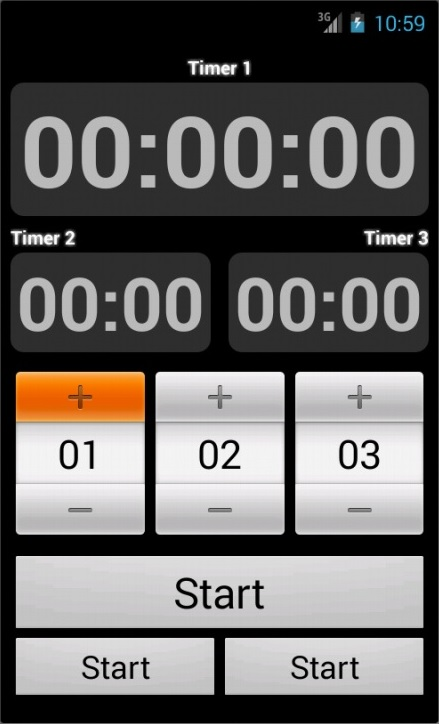
\includegraphics[width=0.18\columnwidth]{figures/before.jpg}
\label{fig:mainTimers}
}
\hfill
\subfloat[\tiny Timer Running]{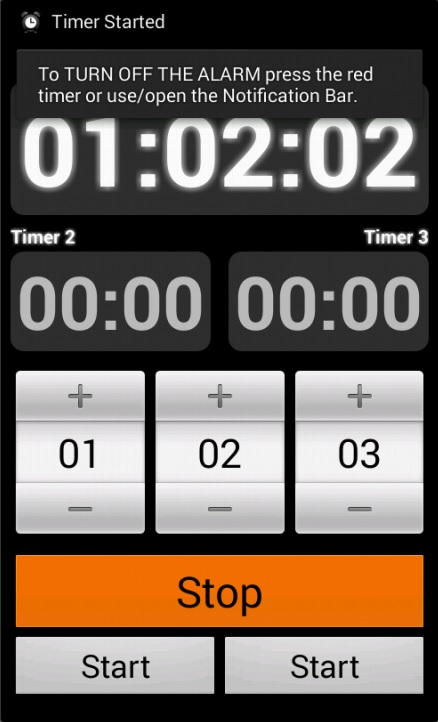
\includegraphics[width=0.18\columnwidth]{figures/timerRunning.jpg}
\label{fig:timerRunning}
}
\hfill
\subfloat[Info]{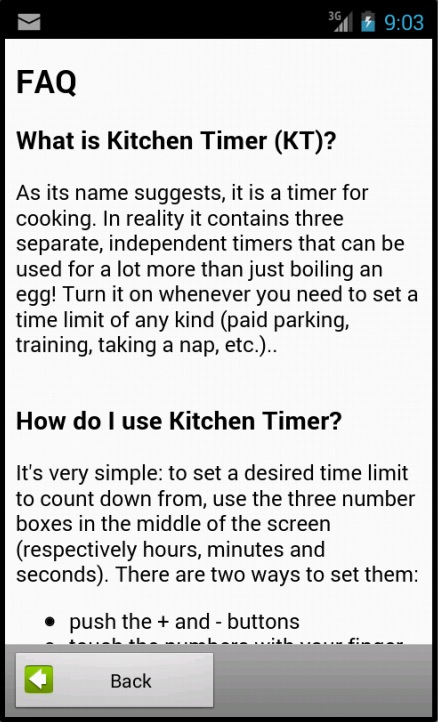
\includegraphics[width=0.18\columnwidth]{figures/info.jpg}
\label{fig:info}
}
\hfill
\subfloat[Preferences]{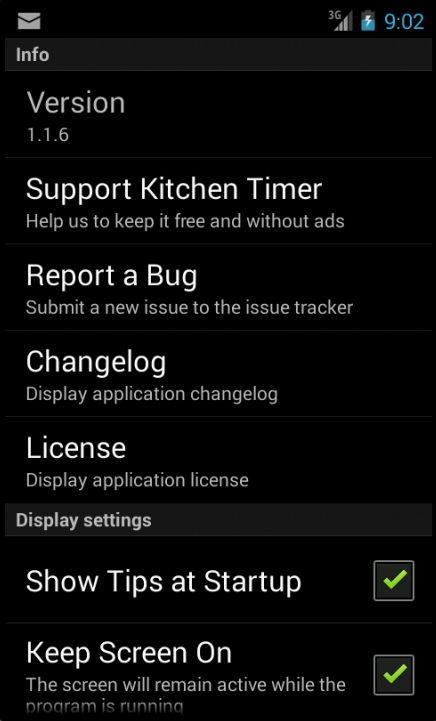
\includegraphics[width=0.18\columnwidth]{figures/prefs.jpg}
\label{fig:prefs}
}
\hfill
\subfloat[Donation]{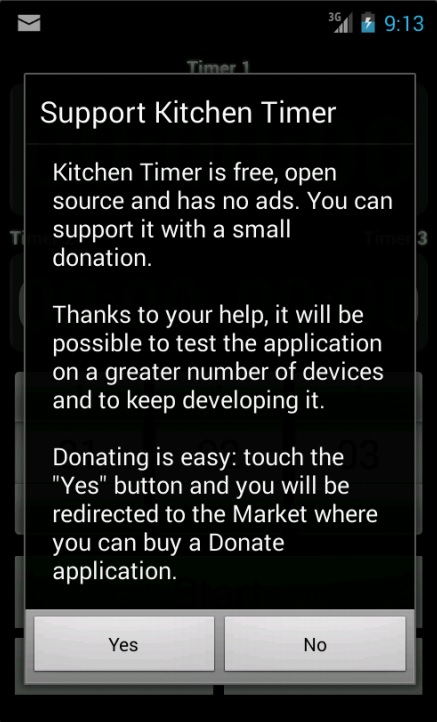
\includegraphics[width=0.18\columnwidth]{figures/donation.jpg}
\label{fig:donation}
}
\Caption{Snapshots of Simplified Kitchen Timer.}
\label{fig:kitchenTimer}
\end{figure}

\begin{figure}[!t]
\centering
\subfloat[The user sets a timer.]{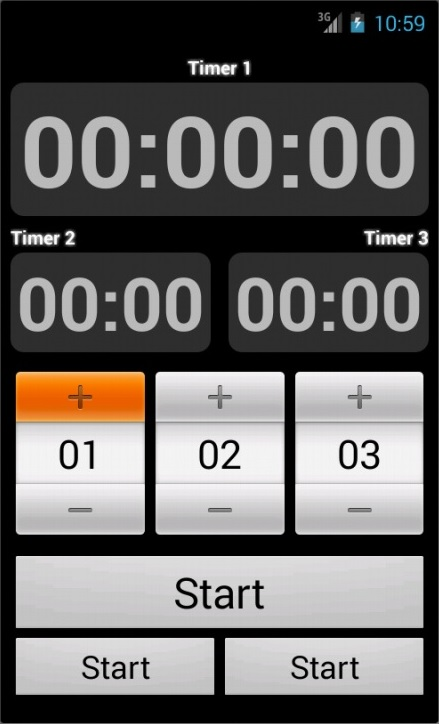
\includegraphics[width=0.3\columnwidth]{figures/before.jpg}
\label{fig:example_c}
}
\hfil
\subfloat[Values overwritten after two rotations.]{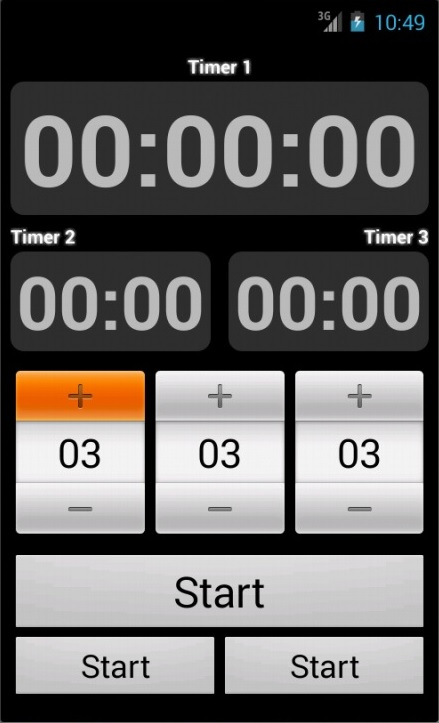
\includegraphics[width=0.3\columnwidth]{figures/after.jpg}
\label{fig:example_d}
}
\Caption{Snapshots of a Bug in Kitchen Timer.}
\label{fig:example}
\end{figure}


As Figure~\ref{fig:example} depicts, Kitchen Timer has a bug that is manifested when the device is rotated twice. If the user sets a timer (Figure~\ref{fig:example_c}), and then rotates the mobile device twice before starting the timer (Figure~\ref{fig:example_d}), the value of seconds overwrites the values of minutes and hours, here changing the timer from 1 hour, 2 minutes, and 3 seconds to 3 hours, 3 minutes, and 3 seconds.
%This bug, similar to most of the rotation bugs we saw in the bug study, is an error of omission, i.e., the programmer neglects that the \texttt{onCreate} method is called after rotation and does not retrieve the data entered into the text box in this method. Hence, traditional adequacy criteria such as 100\% line coverage cannot catch this bug since they focus on errors of commission, i.e., when the programmer does something but incorrectly. GUI based event sequences can, in principle, find such bugs. Yet as apps grow more complicated, event sequences of bigger sizes are required to find bugs, resulting in state space explosion. In addition, automatic test sequence generation techniques which aim these adequacy criteria do not provide automatic oracles, only test sequences. 
Our tool automatically finds this bug. % by particularly noting the fact that, unlike traditional computers, a mobile device can be rotated and is expected to behave properly. 


%This app has an activity life-cycle bug too. The app should show a welcome message the very first time it is run (Figure~\ref{fig:eample_a}). Upon the first launch, the app saves its status in a file to avoid showing the welcome message again (as is commonly done in Android apps). However, the app wrongly uses two different file names for reading and writing. If the app is killed, garbage collected, and restarted, the bug is revealed by showing the welcome message even though it is not the first run, since the app fails to read the status from the file. This is indeed a subtle activity life-cycle bug: It is possible to kill the app (through the \texttt{onDestroy} method) and then restart it before the app gets garbage collected, without manifesting the bug. (The reason is that static variables including the one that keeps the status still have the values they had before killing the app.) Our tool shows this bug by thorough testing of the activity life-cycle. Event sequences, which usually do not include system level events such as killing apps, cannot find this bug. While 100\% line coverage shows this bug, in practice it is rare that full line coverage is achieved. Furthermore, automatic test sequence generation methods that aim such criteria do not provide an automatic oracle and the user has to manually write the oracle/check the results.

\Section{Feature-based Testing of Mobile Apps}
\label{framework}

%Our bug study revealed a number of bug categories that correspond to user-interaction features possible with mobile devices. These features are independent of the logic but tied to GUI states of apps. Such features are present in most mobile apps and there is a common understanding of how an app should support a feature. According to the bug study, examples of features are rotation, activity life-cycle transitions, and gestures. We can identify more features like Android Back button as possible sources of bugs not present in the bug study.

% DECLARE: We describe how to test user-interaction features of mobile apps
The findings of our bug study motivated us to develop an approach for automatically testing user-interaction features (interaction features, or simply features for short throughout the paper) of mobile apps. Our proposed approach is described in this section. We start by defining some terminology.

% PRELIMINARIES
% PRELIMINARIES OF FRAMEWORK SECTION: Currently not a separate sub-section

% Define interaction features
\begin{mydef}[Interaction feature]
\label{def:interactionFeature}
An interaction feature is an action supported by the mobile platform, which enables a human user to interact with a mobile app, using the mobile device and the graphical user-interface (GUI) of the app. Further, an interaction feature is associated with a common sense expectation of how the mobile app should respond to that action. 
\end{mydef}
\vspace*{-2ex}

% Natural language explanation of user-interaction features
Interaction features include actions like rotating a mobile device, general purpose gestures like zooming in/out or scrolling, and actions which start, pause, kill or resume operation of an app, taking its Activity GUI components through various states in their life-cycle. These features were discussed in our bug study. In addition, features like the \textit{Back} or \textit{Up} buttons of the Android platform\footnote{See \url{http://developer.android.com/design/patterns/navigation.html}.} are also valid interaction features. Note that the above definition \textit{excludes} a number of common gestures such as {\small\texttt{click}} or {\small\texttt{longClick}}, or other custom gestures, for which there is no standard expected response from apps; it is completely context and application specific. Since a given interaction feature will have, in general, a standard expected behavior, across apps and different mobile platforms\footnote{Specific apps may of course choose to modify this standard response.}, this provides a general, app agnostic \textit{oracle} for validating an app's response to exercising that feature. Thus, a key component of our approach is authoring such reusable oracles and employing them in interaction feature testing.

% GUI Model and GUI States
We follow a model-driven approach to generating test-cases for testing interaction features of a given mobile app. The starting point for our technique is a finite state model of the GUI behavior of the app, which is defined as follows.

\begin{mydef}[GUI model]
\label{def:GUImodel}
A GUI model of an app is a finite state machine $\mathcal{M}$, denoted by the $4$-tuple $\mathcal{M} = (S, s_0, A, R)$, where $S$ is a finite set of abstract states representing different GUI screens, $s_0 \in S$ is the initial state denoting the app's opening screen, $A$ is a finite set of application specific actions the user may perform in executing the logic of the app, and $R \subseteq S \times A \times S$ is a transition relation describing transitions between states in $S$ in response to user actions from $A$.  
\end{mydef} 
\vspace*{-2ex}

%%%%% INCORPORATE THESE POINTS BELOW
%We identify the following properties for user-interaction features (features for short throughout the paper).
%\begin{itemize}
%\item 
%(1) A user-interaction feature is a way of interacting with the mobile device at the GUI level that is common between apps.
%\item 
%(2) There is an app agnostic \emph{oracle} for a feature. Even though it is possible to redefine how an app responds to exercising a feature, there is a common sense of what should happen in most apps.
%\item 
%(3) In most cases, features are so app agnostic that they are not explicitly included in GUI models. For instance, what happens after killing or pausing an app is rarely included in the GUI model and is usually inferred from the activity life-cycle.
%\item 
%(4) Even though features are usually absent from GUI models, apps have to actually implement feature functionalities and are expected to support features and give the results anticipated by features' oracles.
%\end{itemize}

% Further explanation of GUI Models, GUI models as directed graphs
Two GUI screens are represented by the same abstract state in
$\mathcal{M}$ if and only if they contain the same set of actions on
the same widgets. The only exception to this is screens showing
collections of items, such as books, files, songs, transactions,
\textit{etc.}, where each item supports some set of actions. In this
case two screens with different (non-zero) numbers of items are
interpreted as the same state. Thus, the contents of a collection are
abstracted as empty or non-empty.  Similar notions of GUI states have
also been used in previous work~\cite{Dynodroid:2013,
  collider2013}. The set $A$ includes application specific actions
such as clicks or longClicks, \textit{etc.,} on specific widgets but
\textit{does not} include platform supported interaction features (e.g., device rotation, \textit{etc.}). We
believe this is typical of GUI models as well~\cite{YangFASE2013}.

Note that although the visible part of a GUI screen of a mobile app, as viewed on a mobile device, may change by performing an action such as a device rotation, a zoom, or a scrolling action, these apparently different screens still correspond to the same abstract state in the GUI model. We define the notion of a \textit{view}, denoted by the symbols $w$, to represent the visible portion of abstract GUI model states $s$. Thus, a state $s$ can have several views, generated by exercising different available interaction features on $s$. Specifically, we use the notation $\Phi(s, \mathbf{u}, -)$ and $\Phi(s, \mathbf{u}, +)$ to denote respectively, the two different views of state $s$ before and after action (or action sequence) $\mathbf{u}$ was fired, where $\mathbf{u}$ corresponds to an instance of exercising an interaction feature. The view notation provides a relative notion of \textit{time} of sampling states (for their current view), before and after exercising interaction features.

A GUI model $\mathcal{M}(S, s_0, A, R)$ can also be represented as a rooted, labeled directed graph $G = \langle V, E, r, A, \mathcal{L} \rangle$, in a straightforward manner. Here, the nodes $V$ represent the states $S$, the root node $r$ represents initial state $s_0$, edges $E$ represent transitions between states, consistent with transition relation $R$, and the labeling function $\mathcal{L} \colon E \to A$ labels each edge with the action $a \in A$ responsible for the transition. GUI models can either be constructed manually or generated automatically using one of the techniques from a growing body of work on GUI model generation for mobile apps~\cite{AmalfitanoASE2012, Joorabchi:2012:WCRE, YangFASE2013}.
%to automatically generate tests that exercise features and assert oracles.

% Summarize Overall Approach
\textbf{Overall Approach:} 
Our technique generates compact test suites, complete with test oracles, to comprehensively test interaction features of a given mobile app. The approach uses an extensible library $\mathcal{F}$ of reusable and application agnostic feature definitions, described in Section~\ref{sec:featureDefinition}. Given a user provided GUI model of the app we automatically augment this model with feature instances, using the feature definitions in $\mathcal{F}$ (Section~\ref{sec:modelAugmentation}). %using user feedback to customize the features when needed. 
Then, based on the cost and test adequacy criteria defined in Section~\ref{sec:testSuiteDefinition}, we automatically traverse the augmented model to create compact test sequences (Section~\ref{sec:traversalAlgo}). Finally, we automatically instantiate test oracles in the test sequences to obtain a compact and complete test suite.
%a complete test suite that tests the user-interaction features of the app. 



% FORMAL DEFN. OF FEATURE & EXAMPLES
\Subsection{Authoring Oracles for Interaction Feature Testing}
\label{sec:featureDefinition}

We introduce an extensible framework in which interaction features can be defined in an application agnostic manner and stored in a library. When testing a given app our technique appropriately instantiates features from the library, using these feature definitions, and generates tests, complete with test oracles, to comprehensively test each feature.

\begin{mydef}[Feature definition]
\label{def:feature}
The feature definition of a given interaction feature $f$ is a triple: $\langle \mathbf{u}_f, D_f(s), O_f(w_1, w_2) \rangle$. %we need the following triple: $\langle S_f, A_f, O_f(s_1, s_2, \ldots, s_k) \rangle$. $S_f \subset S$ is a subset of the app's GUI states on which the feature is applicable.
$\mathbf{u}_f = \langle u_1, u_2, \dots, u_n \rangle$ is a sequence of actions that exercises the feature. $D_f(s)$ is the destination function, that maps a given state $s$ at which the feature can be exercised to a set of states $S_f \subseteq S$ that could potentially result from exercising $f$ at state $s$. $O_f(w_1, w_2)$ is the oracle for feature $f$, where $w_1 = \Phi(s_1, \mathbf{u}_f, -)$ is a view of some state $s_1$
before firing actions $\mathbf{u}_f$ and $w_2=\Phi(s_2, \mathbf{u}_f, +)$ is a view of a state $s_2$ reached after firing actions $\mathbf{u}_f$ on some previous state $s_1$, possibly the same state $s_2$.
%$O_f(s_1, s_2, \ldots, s_k)$ is the oracle for feature $f$. It is a boolean predicate over the set of states $s_1, s_2, \ldots, s_k \in S$ which evaluates to \texttt{true} if states $s_1, s_2, \ldots, s_k$ satisfy the specific relationship encoded in the predicate, and \texttt{false} otherwise.
\end{mydef}
\vspace*{-2ex}

A crucial aspect of the above feature definition is to express $\mathbf{u}_f$, $D_f$, and $O_f$ in an application agnostic manner. We demonstrate how to do this below, through example feature definitions of several common interaction features. Another important restriction implied by Definition~\ref{def:feature} is that the set of abstract states in the GUI model should be closed under application of the interaction feature, \ie exercising the feature in one of the states should not take the application to a fundamentally new abstract state outside the GUI model. This common sense restriction is also valid for all interaction features in our knowledge. In the following examples we use $\Phi^-(s)$ and $\Phi^+(s)$ as shorthand for $\Phi(s, \mathbf{u}_f, -)$ and $\Phi(s, \mathbf{u}_f, +)$ respectively, since $\mathbf{u}_f$ is clear from the context.

%In many if not most practical instances, fully automatable oracles typically involve a predicate over two states. For example, the oracle for a double screen rotation\footnote{Rotating the screen $90^\circ$ twice consecutively.} would assert that the application GUI states $s_1$ and $s_2$ that exist before and after the double rotation should be equal, i.e., $(s_1 = s_2)$.

%We introduce an extensible language for defining features oracles ($O_f$'s). One can add to the set of features by identifying the relationship between the expected state and an existing state. For some user-interaction features, the expected state after exercising the feature is exactly the same as a previously seen state. Examples of such features are as follows.

{\bf Double rotation (DR):} We incorporate the mobile device rotation feature in a \textit{double rotation} feature definition, which expresses the act of rotating a mobile device and then rotating it back to the original orientation. With this action the application should stay in the same state. Further, the view of that state before an after double rotation should be identical. This is expressed in the feature definition: $\mathit{DR} = \langle \mathbf{u}_f = \langle rotate, rotate\rangle, D_f(s) = \{s \}, O_f = (\Phi^-(s) = \Phi^+(s)) \rangle$.
%O_f = (\Phi(s, \mathbf{u}_f, -) = \Phi(s, \mathbf{u}_f, +)) \rangle$.
\\
\indent
{\bf Killing and restarting (KR):} The operating system might choose to kill and then restart an app for various reasons (\eg low memory). Similar to double rotation, the app should retrieve its original state and view. Thus, $ \mathit{KR} = \langle \mathbf{u}_f = \langle kill, restart\rangle, D_f(s) = \{s \}, O_f = (\Phi^-(s) = \Phi^+(s)) \rangle$.
\\
\indent
{\bf Pausing and resuming (PR):} The app can be paused (\eg by hitting the Android Home button) and then resumed. $ \mathit{PR} = \langle \mathbf{u}_f = \langle pause, resume\rangle, D_f(s) = \{s \}, O_f = (\Phi^-(s) = \Phi^+(s)) \rangle$. Killing and then restarting, and pausing and then resuming are both instances of activity life-cycle transitions which all apps should support.
\\
\indent
{\bf Back button functionality (Back):} The Back button is a hardware button on Android devices which takes the app to the previous screen. $ \mathit{Back} = \langle \mathbf{u}_f = \langle back \rangle, D_f(s) = \{s_p : s_p \in parent(s) \}, O_f = (\Phi^-(s_1) = \Phi^+(s_1)) \rangle$, where $s_1 \in D_f(s)$. In this case, the destination function produces a set of destinations $D(s)$ corresponding to each of the parent (using the standard graph theoretic notion of parent and child) nodes of the current state $s$ in the GUI model.
\\
%$\langle S_f = S, A_f = \langle a_1, back\rangle, O_f = (s_1 = s_2)\rangle$ where $a_1$ is any navigation action in the app model that takes the app from one screen to another.
\indent
{\bf Opening and closing menus (Menu):} The hardware Menu button on Android devices opens and closes custom menus that each app defines. For this feature definition $\mathit{Menu} = \langle \mathbf{u}_f = \langle menu, menu\rangle, D_f(s) = \{s \}, O_f = (\Phi^-(s) = \Phi^+(s)) \rangle$.

%{\bf Up functionality:} The Up button was introduced in Android 3.0. It appears on the top left corner of the screen and consists of the app icon and a left-point caret. The Up functionality is similar to Back, except that Back always takes the app to the previous screen while Up takes it to the parent screen, which might or might not be the same. As opposed to Back, the model has to define the target of the Up functionality, since it is not uniquely defined and depends on how the hierarchy of screens is viewed. If $s_1$ and $s_2$ are the states before and after hitting the Up icon and $s_3$ is the expected target of Up after $s_1$ according to the model then we have $\langle S_f = S - \{top\}, A_f = \langle up\rangle, O_f = (s_3 = s_2)\rangle$. $top$ is the topmost level screen for which Up is undefined.

%{\bf Double scrolling:} Scrolling down and then back up should bring back the original screen. $\langle S_f = S, A_f = \langle scrollDown, scrollUp\rangle, O_f = (s_1 = s_2)\rangle$.

In the above instances the oracle was always an assertion of equality between two appropriate state views. In general, however, the oracle predicate can include arbitrary relational or logical operators. %For some other user-interaction features, the expected state is a subset or a superset of a previously seen state.
For example:

{\bf Zooming in (ZI):} Zooming into a screen should bring up a subset of what was originally on the screen. $\mathit{ZI} = \langle \mathbf{u}_f = \langle zoomIn\rangle, D_f(s) = \{s \}, O_f = (\Phi^-(s) \supset \Phi^+(s)) \rangle$.
\\
\indent
{\bf Zooming out (ZO):} Zooming out from a screen should result in a superset of the original screen. $\mathit{ZO} = \langle \mathbf{u}_f = \langle zoomOut\rangle, D_f(s) = \{s \}, O_f = (\Phi^-(s) \subset \Phi^+(s)) \rangle$.
\\
%The user can extend the set of user-interaction features by defining new oracles. For instance:
\indent
{\bf Scrolling (SCR):} Scrolling down (or up) should display a screen that shares parts of the previous screen. $\mathit{SCR} = \langle \mathbf{u}_f = \langle scrollDown\rangle, D_f(s) = \{s \}, O_f = (\Phi^-(s) \cap \Phi^+(s) \neq \emptyset) \rangle$.
%$\langle S_f = S, A_f = \langle scrollDown\rangle, O_f = (s_1 \cap s_2 = \emptyset (or \neq \emptyset)))\rangle$.
%Previous work \remark{ref?} showed bugs that would make the app run out of memory in case of many scrolls.

Note that the feature definition itself includes an implementation of the oracle, albeit an app independent one, that can be re-used across different apps. Thus, the semantics of operators used in the oracles are defined there.


% GUI MODEL AUGMENTATION USING FEATURE LIBRARY
\subsection{Augmenting GUI Models with Feature Instantiations}
\label{sec:modelAugmentation}

Given a GUI model $G = \langle V, E, r, A, \mathcal{L} \rangle$ of the target app and a library $\mathcal{F}$ of interaction features, specified as discussed in Section~\ref{sec:featureDefinition}, the next step in our approach is to annotate $G$ with all possible instantiations of each feature in $\mathcal{F}$ to produce an augmented GUI model $G^+ = \langle V, E^+, r, A^+, \mathcal{L}^+ \rangle$. Specifically, this involves adding a set of special labeled edges, called \textit{golden edges}, to $G$. Each golden edge, $e_f(v_1, v_2)$ denotes that feature $f$ when exercised at the state of vertex $v_1$ takes the application to the state of vertex $v_2$. Further, $e_f$ is labeled with $\mathbf{u}_f$, the action sequence of feature $f$. Thus, the augmented model $G^+$ includes the augmented set of edges $E^+ = E \cup E_{golden}$,  augmented action set $A^+ = A \cup \bigcup_{f \in \mathcal{F}} \mathbf{u}_f$, and appropriately modified labeling function $\mathcal{L}^+: A^+ \rightarrow E^+$, where $E_{golden}$ are the golden edges and $\bigcup_{f \in \mathcal{F}} \mathbf{u}_f$ are the actions for features $\mathcal{F}$ labeling the golden edges.

\begin{algorithm}[t]
\begin{footnotesize}
  \DontPrintSemicolon
  \SetAlFnt{\scriptsize\scriptfont}
  \SetKwData{Left}{left}\SetKwData{This}{this}\SetKwData{Up}{up}
  \SetKwFunction{Union}{Union}\SetKwFunction{FindCompress}{FindCompress}
  \SetKwInOut{Input}{Input}\SetKwInOut{Output}{Output}
  \caption{GUI Model Augmentation Algorithm}\label{alg:augmentGUImodel}
  \Input{$G = \langle V, E, r, A, \mathcal{L} \rangle$: Original GUI model of target app \\
  	$\mathcal{F}$: Feature library
  }
  \Output{$G^+ = \langle V, E^+, r, A^+, \mathcal{L}^+ \rangle$: Augmented GUI model}
  \BlankLine
  \Begin{
  		$G^+ \leftarrow G$\;
  		\ForEach{$v \in V$}{
  			\tcp{Iterate over each vertex (state) of $G$}
  			\ForEach{$f \in \mathcal{F}$}{
  				\tcp{Iterate over each feature in $\mathcal{F}$}
  				$dSet = \mathit{destinationSet}(v, G^+, f) $\;
  				\ForEach{$v_1 \in dSet$}{
  					$e \leftarrow \mathit{createEdge}(v, v_1);$\;
  					$\mathit{setEdgeLabel}(e, getAction(f))$\;
  					$\mathit{markGolden}(e)$\;
  					$\mathit{addEdge}(e, G^+)$\;
  				}
  			}
  		}
			\Return{$G^+$}\;
  }
\end{footnotesize}  
\end{algorithm}

Algorithm~\ref{alg:augmentGUImodel} shows the procedure to perform GUI model augmentation. The algorithm iterates over each state $v$ in the GUI model (lines $3-13$) and each feature $f$ in library $\mathcal{F}$, instantiating $f$ at $v$, as per the feature definition. It computes the set of possible destination vertices $dSet$, by evaluating function $D_f$ in the feature definition (function $\mathit{destinationSet()}$ on line $5$). It then iterates over each possible destination vertex $v_1$ (lines $6-11$) creating and adding a golden edge, labeled by the feature's action sequence $\mathbf{u}_f$ (line $8$), to the augmented model $G^+$.
Figure~\ref{fig:dotGraph} shows the GUI model of our simplified version of Kitchen Timer from Section~\ref{example}, augmented with golden edges for the Double Rotation and Back button features.

\begin{figure*}[!t]
\centering
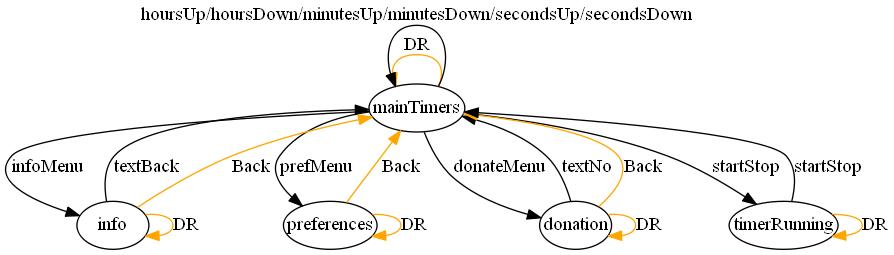
\includegraphics[width=0.65\textwidth]{figures/dotGraph.jpg}
\caption{Simplified Model of Kitchen Timer.}
\label{fig:dotGraph}
\end{figure*}


% TEST SUITE DEFINITION (test case, covering features through test cases, test-suite cost function)
\subsection{Test Suite Definition}
\label{sec:testSuiteDefinition}

Given an augmented GUI model $G^+$ the final phase of our technique generates a test suite with the following goal.

\noindent\textbf{Test objective:} \textit{A \textbf{compact} suite of tests to \textbf{comprehensively} test the interaction features of the given app under test.}

 A test is a sequence of actions (\ie a sequence of edges or a path in $G^+$) starting at the initial state $r$, with each action possibly followed by an oracle check. Therefore, a test can be represented as $\langle a_1, o_1, \dots, a_n, o_n \rangle$. Each $a_i \in A^+$ is any action (including those that exercise interaction features) allowed by the app's GUI. Each $o_i$ is either an oracle check or no operation. We assume that oracle checks are side effect free, \ie they do not change the state of the app.

We define a test adequacy criterion to concretize the notion of a ``comprehensive" test suite stated in the test objective. Since mobile apps are event-driven systems and interaction features are elements of the app's GUI, we develop a criterion that is motivated by the notions of path coverage and event-flow coverage used by previous work on GUI testing~\cite{memon2001coverage}. This is in contrast to code coverage-based criteria such as line or branch coverage, which would be more appropriate for functional testing of the software implementation rather than testing its high level platform features, as in our case. Intuitively, we say that a test suite covers a feature, if it contains tests to exercise and validate \textit{each possible instance} of exercising that feature on that app. Simply put, this implies exercising the feature in each GUI state. Given a test suite $T$, an interaction feature $f$ from a feature library $\mathcal{F}$ and an augmented GUI model $G^+ = \langle V, E^+, r, A^+, \mathcal{L}^+ \rangle$, as defined in Section~\ref{sec:modelAugmentation}, we define adequacy of $T$ in testing $f$ with respect to $G^+$ as follows.

\begin{mydef}[Interaction feature coverage]
\label{def:coverage}
A test suite $T$ covers a feature $f$ iff $\forall s \in S: \exists t \in T, t = \langle a_1, o_1, \dots, a_n, o_n  \rangle, \exists j, k, 0 \leq j < k \leq n$ such that $\langle a_1, \dots, a_j \rangle$ takes the app from the initial state $s_0$ to state $s$, $\langle a_{j+1}, \dots, a_k \rangle = \mathbf{u}_f$, and $o_k = O_f$.
\end{mydef}

Since there are no standard or widely accepted cost functions to optimize test suites we quantify the ``compactness"  of our test suite using the common sense observation that large test suites are hard to set up, execute, and maintain. The size of a test suite can be measured by the number of tests it contains as well as the cumulative number of operations (actions $a_i$) in the test suite as a whole.
We propose a customizable cost function that captures this.

%intuitively measures the time it takes to execute a test suite, including the set up and execution times. 
%Then we show how to leverage this cost function to traverse the model more effectively, in order to get smaller and faster to run test suites.

\begin{mydef}[Cost of a test suite]
\label{def:costfunction}
The cost of a test suite T is $cost(T) = \alpha * |T| + \beta * \Sigma_{t \in T} |t|$, where $\alpha$ and $\beta$ are positive co-efficients. \end{mydef}

Coefficient $\alpha$ measures the relative cost of developing and maintaining a suite, which scales with the number of tests in a suite. Coefficient $\beta$ quantifies the cost of executing actions and asserting oracles which is proportional to the number of operations.


% TEST SUITE GENERATION
\Subsection{Feature-based Test Sequence Generation}
\label{sec:traversalAlgo}

Recall that interaction features are orthogonal to the core logic of the app and their function is typically to help the user navigate or access content on the app by mutating the state of the app's GUI. Further, exercising an interaction feature on a given state has no side effects in terms of the GUI model, \ie the effect of exercising that feature is limited to a single GUI screen and has no impact on the downstream actions. This observation is very important as it allows us to arbitrarily mix and match instances of several features (and their test oracles) in a single test case, as long as it lowers the cost of the test suite, per Definition~\ref{def:costfunction}. Since each instance of every feature is already recorded in our augmented GUI model $G^+$ (servicing the test adequacy criterion of Definition~\ref{def:coverage}), our test generation problem can be stated as follows.

\noindent\textbf{Test suite generation problem:} \textit{Given an augmented GUI model $G^+$ generate a minimum cost test suite such that each golden edge in $G^+$ is covered by at least one test in the suite.}

%\begin{proof}
%The proof sketch is by reducing the \textit{minimum path cover problem}~\cite{PathCover:NtafosH79} to this problem as follows. Given an instance of the minimum path cover problem, take the given directed graph $G$ and construct a modified $G'$ from it:
%\begin{enumerate}
%\item Add a self loop to every vertex and mark it as golden (ensuring that we cover all golden edges if and only if we cover all vertices).
%\item Add a new root node $r$ and add an edge from $r$ to each vertex of $G$ (accounting for the fact that in the original path cover problem paths need not originate at a starting node, which they do in our case).
%\end{enumerate}
%Now we solve our problem on $G'$ with $\alpha = 1$ and $\beta = 0$, thus minimizing the number of $r$-originating paths covering all golden edges, or essentially all vertices, irrespective of path lengths. The answer would be a minimum path cover over $G$.
%\end{proof}

It can be shown that the above problem is NP-hard, by reducing the \textit{minimum path cover problem}~\cite{PathCover:NtafosH79} to this problem. We omit the detailed proof here for lack of space.

We propose a greedy algorithm for this NP-hard problem. In addition, we introduce two optimizations to further reduce the cost associated with covering features. Algorithm~\ref{alg:traversalAlgo} shows a pseudo-code of the traversal algorithm we propose. The input to this algorithm is the augmented graph model. We use a set to keep track of \emph{covered edges} $CE$ and a stack to record the test sequence. First, on Line~\ref{line:BFS}, we sort the nodes based on their increasing distance from the root using a Breadth First Search (BFS) and keep the sorted list in $L$. For example, we can sort the nodes of Figure~\ref{fig:dotGraph} as $\langle$\emph{mainTimers}, \emph{info}, \emph{preferences}, \emph{donation}, \emph{timerRunning}$\rangle$. Then, working through the list $L$ on Line~\ref{line:loopForL}, we select the next node $s$ that has uncovered outgoing edges (Line~\ref{line:sHasOutgoing}). In our example, the first node in the list with uncovered outgoing edges is \emph{mainTimers} (as we have not yet covered any edges). We use the shortest path from the root to this node (saved through previously performed BFS) as the prefix of all sequences to be generated starting from it. Lines~\ref{line:prefixBeg} to \ref{line:prefixEnd} iterate through the shortest path and (1) mark edges as visited by adding them to $CE$, and (2) push them onto $stack$. The rationale behind using such a prefix is to minimize the cost associated with taking edges to get to a given node, where the exploration for uncovered golden edges begins. % In the case of \emph{mainTimers}, the prefix would be empty as \emph{mainTimers} is the root of the graph.

%\lstinputlisting[caption=Traversal Algorithm in Java.,label=lst:traversalAlgo]{listings/traversalAlgo.java}
\begin{algorithm}[t]
\begin{footnotesize}
  \DontPrintSemicolon
  \SetAlFnt{\scriptsize\scriptfont}  
  \SetKwData{Left}{left}\SetKwData{This}{this}\SetKwData{Up}{up}
  \SetKwFunction{Union}{Union}\SetKwFunction{FindCompress}{FindCompress}
  \SetKwInOut{Input}{Input}\SetKwInOut{Output}{Output}  
  \caption{Traversal Algorithm}\label{alg:traversalAlgo}
  \Input{$G^+ = \langle V, E^+, r, A^+, \mathcal{L}^+ \rangle$: Augmented GUI model of app}
  \Output{$T$: Test Suite}
  \BlankLine
  \Begin{
  		$CE \leftarrow \emptyset$\;
  		$stack \leftarrow \emptyset$\;
  		$L \leftarrow \mathit{sortWithBFS}(G^+)$\;\nllabel{line:BFS}
  		\ForEach{$s \in L$}{\nllabel{line:loopForL}
  			\While{$\exists (s,y) \in outGoing(s), s.t. (s,y) \in E-CE$}{\nllabel{line:sHasOutgoing}
  				\ForEach{$e \in shortestPathBFS(r,s)$}{\nllabel{line:prefixBeg}
  					$stack.push(e)$\;
  					$CE \leftarrow CE \cup \{e\}$\;
  				}\nllabel{line:prefixEnd}
  				$c \leftarrow s$\;
  				$stop \leftarrow false$\;
  				\While{$!stop$}{\nllabel{line:loopForTraversalBeg}
  					\If{$\exists (c,v) \in outGoing(c), s.t. (c,v) \in E-CE$}{\nllabel{line:cHasOutgoing}
  						$CE \leftarrow CE \cup \{(c,v)\}$\;\nllabel{line:coverIt}
  						$stack.push((c,v))$\;\nllabel{line:pushIt}
  						$c \leftarrow v$\;\nllabel{line:updateC}
  					}\lElse{$stop \leftarrow true$\;\nllabel{line:stopToTrue}}
  				}\nllabel{line:loopForTraversalEnd}
  				$T \leftarrow T \cup stack$\;
  				$stack.clear()$\;
  			}
  		}
  		\Return{$T$}\;
	}
\end{footnotesize}  
\end{algorithm}

Then, using $c$ as a pointer to the \emph{current} node, which is initially set to $s$, on Line~\ref{line:cHasOutgoing} we pick an uncovered edge going out of $c$. We take this edge, mark it as covered (Line~\ref{line:coverIt}), push it onto $stack$ (Line~\ref{line:pushIt}), and update $c$ to the destination of this edge accordingly (Line~\ref{line:updateC}). Once we get to a node that has no uncovered outgoing edge, the current test sequence is complete and we set $stop$ to {\small\texttt{True}} on Line~\ref{line:stopToTrue}. The current $stack$ makes one test sequence and we continue by generating more sequences and adding them to $T$ which is the test suite and is the output of this algorithm. For instance, the first test sequence that is generated is shown as $T_0$ under \emph{No Optimization} in Table~\ref{tab:tests}. This Table displays the test suite our greedy algorithm generates for the simplified model of Kitchen Timer. The test suite has $7$ tests at a total cost of $34$, with $\alpha$ and $\beta$ both set to $1$ in the cost function.

\begin{table}
\vspace*{-2ex}
\Caption{Test Sequences for Figure~\ref{fig:dotGraph}.}
\label{tab:tests}
\begin{center}
\begin{tabular}{@{}l@{}l@{}}
\toprule
\textbf{No Optimization}\\
\midrule
\multicolumn{2}{@{}l@{}}{
$T_0$ = $\langle$hoursUp, hoursDown, minutesUp, minutesDown, secondsUp, secondsDown,}\\
\multicolumn{2}{@{}l@{}}{
infoMenu, textBack, prefMenu, Back, donateMenu, textNo, startStop, startStop, DR$\rangle$}\\
$T_1$ = $\langle$infoMenu, Back$\rangle$&
$T_2$ = $\langle$infoMenu, DR$\rangle$\\
$T_3$ = $\langle$prefMenu, DR$\rangle$&
$T_4$ = $\langle$donateMenu, Back$\rangle$\\
$T_5$ = $\langle$donateMenu, DR$\rangle$&
$T_6$ = $\langle$startStop, DR$\rangle$\\
\#Tests = 7, Cost(T) = 34\\
\midrule
\textbf{Prioritization Optimization On}\\
\midrule
\multicolumn{2}{@{}l@{}}{
$T_0$ = $\langle$DR, hoursUp, hoursDown, minutesUp, minutesDown, secondsUp, secondsDown,}\\
\multicolumn{2}{@{}l@{}}{
infoMenu, Back, prefMenu, Back, donateMenu, Back, startStop, DR, startStop$\rangle$}\\
$T_1$ = $\langle$infoMenu, DR, textBack$\rangle$&
$T_2$ = $\langle$prefMenu,	DR$\rangle$\\
$T_3$ = $\langle$donateMenu, DR, textNo$\rangle$\\
\#Tests = 4, Cost(T) = 28\\
\midrule
\textbf{Prioritization and Truncation Optimizations On}\\
\midrule
\multicolumn{2}{@{}l@{}}{
$T_0$ = $\langle$DR, hoursUp, hoursDown, minutesUp, minutesDown, secondsUp, secondsDown,}\\
\multicolumn{2}{@{}l@{}}{
infoMenu, Back, prefMenu, Back, donateMenu, Back, startStop, DR$\rangle$}\\
$T_1$ = $\langle$infoMenu, DR$\rangle$&
$T_2$ = $\langle$prefMenu,	DR$\rangle$\\
$T_3$ = $\langle$donateMenu, DR$\rangle$\\
\#Tests = 4, Cost(T) = 25\\
\bottomrule
\end{tabular}
\end{center}
\vspace*{-0.1in}
\end{table}

We introduce two optimizations to augment our basic traversal algorithm. The first optimization called \textit{prioritization}, prioritizes golden edges whenever there are both golden and regular (non-golden) uncovered edges going out of a node, since the goal of the traversal algorithm is to cover golden edges. To implement this optimization, the method $outGoing()$ in Algorithm~\ref{alg:traversalAlgo} returns golden edges first. Table~\ref{tab:tests} displays the output of the traversal algorithm with this optimization incorporated. For example, at the beginning of \emph{$T_0$} under \emph{Prioritization Optimization On}, when the golden edge \emph{DR} is available, it is taken before any other edge. This optimization makes the test suite smaller and decreases the cost from $34$ to $28$.

The second optimization, called \textit{truncation}, uses the observation that a test can be truncated after the last golden edge it covers, and deleted if it covers no golden edges. Truncation is applicable in a post-processing phase on any test suite. Table~\ref{tab:tests} shows the result of combining both optimizations (applying truncation on the result of prioritization optimization) which makes the cost of the test suite go down to 25.

Once test sequences are generated, we insert oracles by augmenting test sequences in two ways.
Firstly, we automatically add appropriate instrumentation before and after relevant actions in test sequences, to dynamically record %details of the app 
the current view of each GUI state, as the test is being run. Secondly, we automatically instantiate oracles $O_f$ from the feature definitions to assert checks on the state views recorded by the instrumentation.


% TOOL
\subsection{Implementation}

The \tool{} tool embodies our approach.  \tool{} currently supports
testing of the following features\footnote{Zooming in and out
  functionality is currently unavailable in JUnit and Robotium
  frameworks, hence we did not include them in our tool.}: rotation,
killing and restarting, pausing and resuming, and Back button.
{}
There are four key steps in using \tool.
\\
%\begin{enumerate}
\indent
{\bf Step 1:} \tool{} receives a (manually or automatically generated)
model of the application's GUI as an XML file. \tool{} automatically
adds golden edges for the currently supported set of features.
%(rotation, killing and restarting, pausing and resuming, and Back button)
Then, \tool{} generates a graphical representation of the GUI
model using the dot program\footnote{\url{http://www.graphviz.org}} so that
the user can visually validate the model. Figure~\ref{fig:dotGraph} is
a sample graphical representation that \tool{} generated.
\\
\indent
{\bf Step 2:}
Once the model is validated, \tool{} traverses the model using traversal algorithms to generate test suites. \tool{} provides the following options for traversing the model: (1) our algorithm described in Section~\ref{sec:traversalAlgo} and (2) a basic Depth First Search algorithm (DFS) that covers all edges to serve as a baseline for comparison. On top of our traversal algorithm, each of the optimizations can be turned on or off independently. By traversing the model, \tool{} generates a suite of JUnit\footnote{\url{http://junit.org}} tests. The tests use a combination of Robotium\footnote{\url{https://code.google.com/p/robotium}} and JUnit to interact with Android~apps.
\\
\indent
{\bf Step 3:}
In the generated test suite, \tool{} automatically inserts (1) instrumentation to record views of states, and (2) oracles after exercising each golden edge.
Recording views of states can be done through various user-interfaces provided by a mobile platform. We experimented with two interfaces from the Android platform: Hierarchy Viewer\footnote{\url{http://developer.android.com/tools/help/hierarchy-viewer.html}} and taking graphical snapshots.
\\
\indent
Hierarchy Viewer is a tool for debugging user-interfaces of apps that displays the hierarchy and properties of items on the screen.
%of the mobile device or emulator, their hierarchy, and their properties.
A programmatic interface is not available for Hierarchy Viewer to be used by tests, so we implemented one using Java reflection. We used this implementation to assert oracles that compare the hierarchy and properties of items on the screen, provided by the state view.
This implementation of Hierarchy Viewer included iterating over all items on the screen and fetching the values of their public fields through calling all of their public get methods. However, we did not proceed with Hierarchy Viewer, because it has multiple drawbacks. Firstly, it is prone to false positive, since there are many public variables that are irrelevant to what is displayed on the screen. For example, the  \emph{getDrawingTime} method of an item shows how long it took to draw on the screen, which varies from time to time and falsely alarms difference between two views that are indeed the same. Secondly, it is relatively slow, since there might be many nested items on the screen each having various public variables.
\\
\indent
Graphical snapshots are taken from inside JUnit tests and are then compared using image processing. In the current implementation of \tool{}, snapshots of the state views are automatically recorded and the comparison is based on a basic image differencing algorithm that uses the Red-Green-Blue coloring system to compare images pixel by pixel and allows for an adjustable threshold of difference.
%Listing~\ref{lst:sampleTest} shows the simplified version of a sample JUnit test that \tool{} generated for Kitchen Timer. The \emph{imagesEqual} method contains the basic image comparison algorithm.
Listing~\ref{lst:imageComparison} shows the \emph{imagesEqual} method from a sample JUnit test which contains the basic image comparison algorithm.
Since the views are rendered on the same device and the same screen, it is conceivable that basic image comparison might be good enough. Indeed, taking graphical snapshots proved to be easier to use than Hierarchy Viewer for the currently implemented set of features, gave less false positives, and was faster.
\\
%\lstinputlisting[caption=Example Test Generated by \tool.,label=lst:sampleTest]{listings/sampleTest.java}
\lstinputlisting[caption=Image Comparison Method that \tool{} Uses.,label=lst:imageComparison]{listings/imageComparison.java}

\indent
%Of course, one can use any other tool to record the view of the app, as long as the recording can be programmatically performed by test sequences and a method is provided for comparing state views. Such different tools might be more appropriate for implementing an extended sets of features, e.g., zooming and scrolling.
\\
\indent
{\bf Step 4:}
Now the test suite is complete and can be run to test the app running on an Android device or emulator.
Each test case traverses and checks multiple golden edges. After executing each test, a log is provided which contains the result of checking each golden edge as Pass or Fail. In addition, \tool{} takes snapshots of the app and provides them along with the expected snapshot for each failure. These snapshots facilitate identifying false positives, evaluating the severity of bugs, and debugging.
%\end{enumerate}


\section{Evaluation}
\label{evaluation}

We evaluated \tool{} on $\NumApps$ Android apps ($3$ apps from previously studied apps and $3$ apps from the apps
we selected, as discussed in Section~\ref{study}) to answer the
following research questions (RQ):
\begin{enumerate}
\item 
%(1) 
Can \tool{} find bugs in real applications?
\item 
%(2) 
How effective is \tool{} in terms of the ratio of real bugs to false positives (FP's)?
\item 
%(3) 
How compact are the test suites generated by \tool?
\end{enumerate}

\subsection{RQ 1 and 2: Finding Real Bugs}
Given manually created GUI models, we used \tool{} to automatically
generate test suites. We first used our traversal algorithm with both optimizations, along with
the image processing oracle. Then, we automatically executed the test
suites on a rooted Android emulator (running Android 4.3 API level 18
with an Intel Atom (x86) CPU, 512 MB of SD card, and resolution
WVGA800).

\begin{table}[t!]
\centering
\caption{Bugs Automatically Found with \tool.}
\label{table:bugsFound}
{
\begin{tabular}{lrrrrrrr}
\toprule
\bf{Application}&\begin{sideways}\bf{\#Tests}\end{sideways}&\begin{sideways}\bf{\#Assertions}\end{sideways}&\begin{sideways}\bf{\#Failures}\end{sideways}&\begin{sideways}\bf{\#FP's}\end{sideways}&\begin{sideways}\bf{\#Bugs}\end{sideways}&\begin{sideways}\bf{\#Distinct FP's}\end{sideways}&\begin{sideways}\bf{\#Distinct Bugs}\end{sideways}\\
\midrule
\textit{Notepad (Version N/A)}&8&22&7&4&3&2&2\\
\textit{OpenSudoku (Version 1.1.5)}&7&22&9&4&5&2&3\\
\textit{Nexes Manager (Version 2.1.8)}&15&67&11&3&8&2&7\\
\midrule
\textit{VuDroid (Version 1.4)}&6&16&3&0&3&0&2\\
\textit{Kitchen Timer (Version 1.1.6)}&8&37&13&5&8&2&4\\
\textit{K9Mail (Version 4.317)}&16&53&8&1&7&1&4\\
\midrule
\bf{Total}&\bf 60&\bf 217&\bf 51&\bf 17&\bf 34&\bf 9&\bf 22\\
\bottomrule
\end{tabular}
}
\end{table}


Table~\ref{table:bugsFound} summarizes the results of finding bugs.
\emph{\#Tests} is the size of the test suite generated for each app
using our traversal algorithm with both truncation and prioritization
optimizations. Each test covers several golden edges and tests multiple features, 
thereby generating compact test suites.
\emph{\#Assertions} shows the total number of assertions in the test
suite, which is equal to the number of golden edges. \emph{\#Failures} is the number of assertions that failed. We
manually investigated the failures and identified real bugs and false
positives. Some of these bugs or false positives were revealed more
than once. Therefore, we show the number of distinct false positives
and bugs in the last two columns.

\tool{} found a total of \NumBugs{} bugs in \NumApps{} apps. These bugs included $12$ rotation bugs, $1$ killing and restarting bug, $5$ pausing and resuming bugs, and $4$ Back button bugs. Examples of the bugs are as follows.

%\noindent
{\bf Pausing and resuming bug in K9Mail}: The user finally finds an
email after searching the inbox for some time, but while reading the
email he receives a phone call (which pauses K9Mail). After the phone
call is over, K9Mail resumes, but back to the inbox, requiring to perform the
search again. Figure~\ref{fig:bug19} depicts this bug. We reported this bug as issue 5926 to K9Mail.
\begin{figure*}[!t]
\centering
\begin{minipage}{.8\columnwidth}
%0.225=0.18/0.8
\subfloat[An open email.]{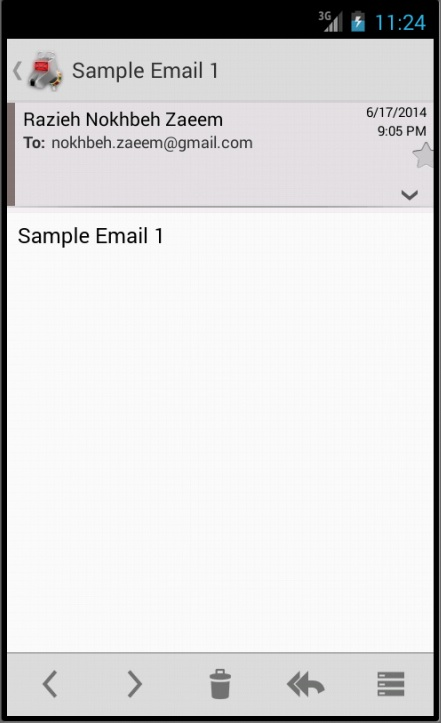
\includegraphics[width=0.225\columnwidth]{figures/bug19/bug19_shot1.jpg}
}
\hfill
\subfloat[A phone call pauses K9Mail.]{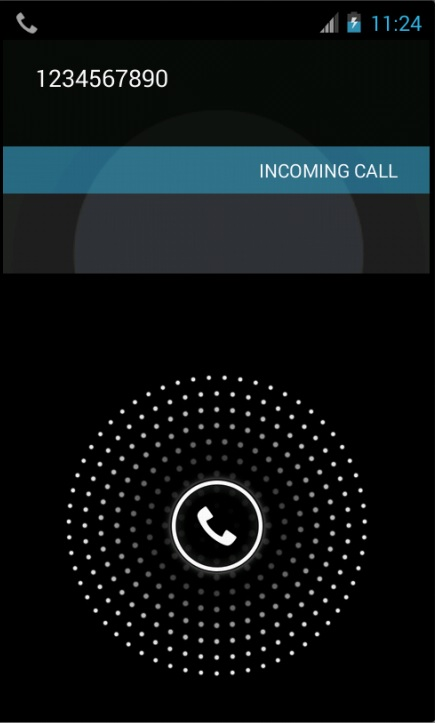
\includegraphics[width=0.225\columnwidth]{figures/bug19/bug19_shot2.jpg}
}
\hfill
\subfloat[K9Mail resumes to the inbox instead of the email.]{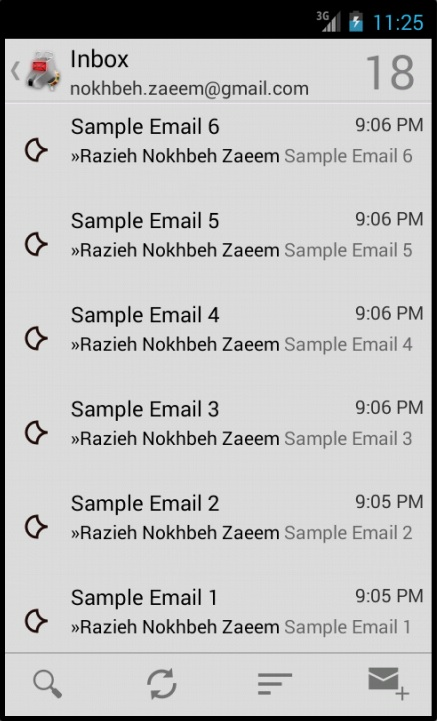
\includegraphics[width=0.225\columnwidth]{figures/bug19/bug19_shot3.jpg}
}
\caption{Pausing and Resuming Bug in K9Mail.}
\label{fig:bug19}
\end{minipage}
\end{figure*}

\indent{\bf Killing and restarting bug in K9Mail}: The operating system decides to kill K9Mail because of low memory while the user is composing an email. K9Mail fails to save the email as a draft, deleting the contents of the email (Figure~\ref{fig:bug17}). We found this bug already reported as issue 161.
\begin{figure*}[!t]
\centering
\begin{minipage}{.8\columnwidth}
%0.225=0.18/0.8
\subfloat[Initially no drafts saved.]{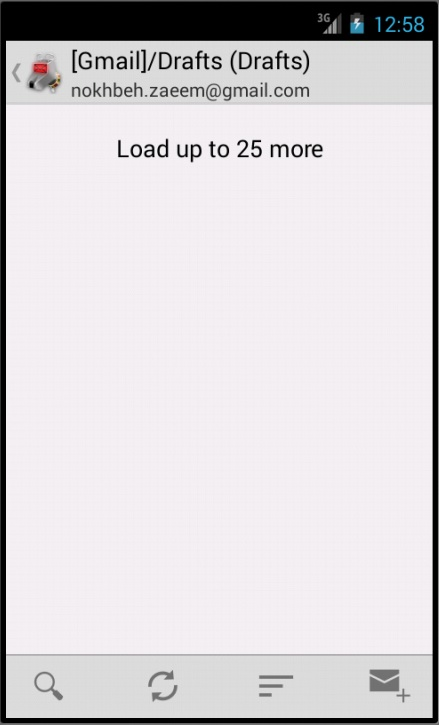
\includegraphics[width=0.225\columnwidth]{figures/bug17/bug17_shot1.jpg}
}
\hfill
\subfloat[While composing an email, the OS kills K9Mail.]{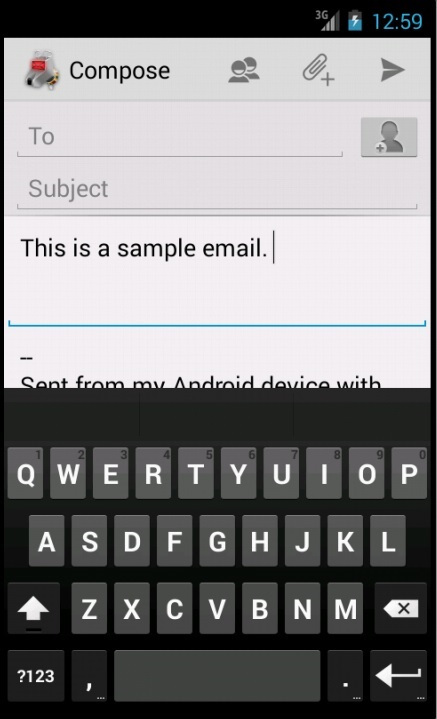
\includegraphics[width=0.225\columnwidth]{figures/bug17/bug17_shot2.jpg}
}
\hfill
\subfloat[K9Mail fails to save a draft.]{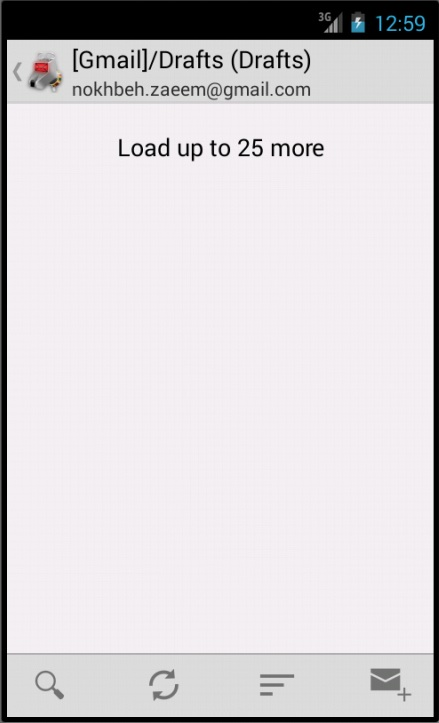
\includegraphics[width=0.225\columnwidth]{figures/bug17/bug17_shot3.jpg}
}
\caption{Killing and Restarting Bug in K9Mail.}
\label{fig:bug17}
\end{minipage}
\end{figure*}

\indent{\bf Rotation bug in Kitchen Timer}: Explained in Section~\ref{example}. We reported this bug as issue 147 to Kitchen Timer.
\\
\indent{\bf Rotation bug in OpenSudoku}: Rotating the device closes the custom pop up for entering numbers and discards them (Figure~\ref{fig:bug25}). We reported this bug as issue 175 to OpenSudoku.
\begin{figure*}[!t]
\centering
\begin{minipage}{.8\columnwidth}
%0.225=0.18/0.8
\subfloat[Before entering numbers.]{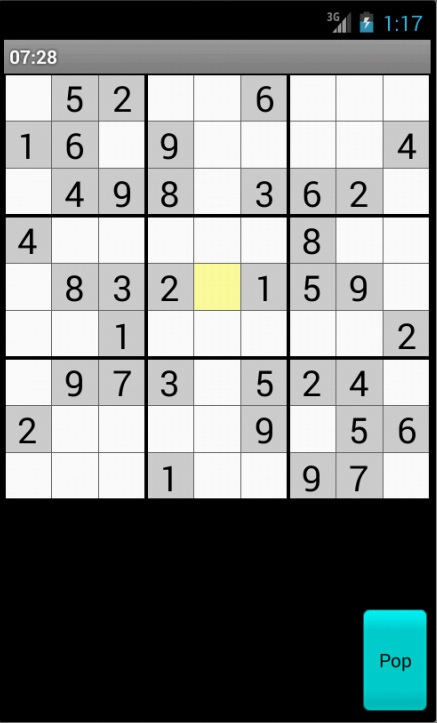
\includegraphics[width=0.225\columnwidth]{figures/bug25/bug25_shot1.jpg}
}
\hfill
\subfloat[Pop up for entering multiple numbers.]{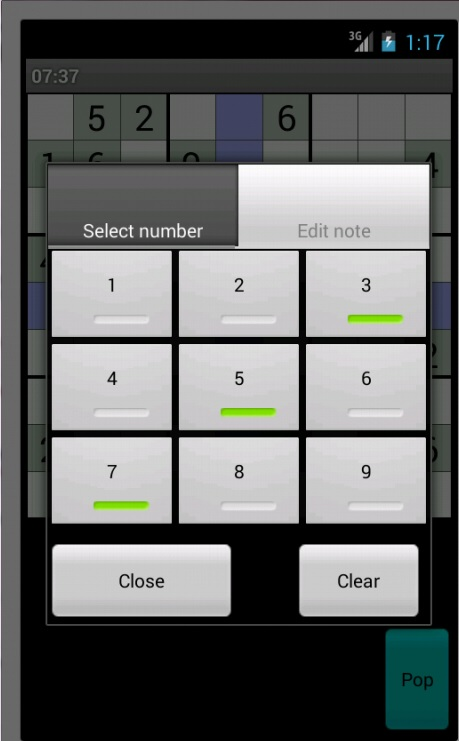
\includegraphics[width=0.225\columnwidth]{figures/bug25/bug25_shot2.jpg}
}
\hfill
\subfloat[Entered numbers discarded after two rotations.]{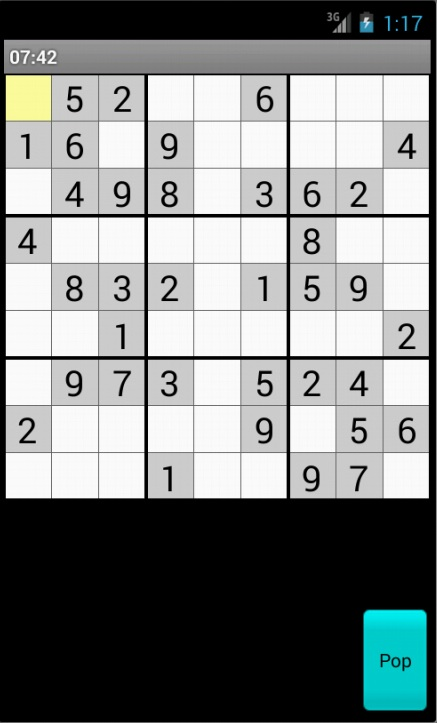
\includegraphics[width=0.225\columnwidth]{figures/bug25/bug25_shot3.jpg}
}
\caption{Rotation Bug in OpenSudoku.}
\label{fig:bug25}
\end{minipage}
\end{figure*}

\indent{\bf Rotation bug in VuDroid}: Rotation clears tab selection. As Figure~\ref{fig:bug9} displays, the default tab is the Browse tab. If the user selects the Recent tab and then rotates the device, the tab selection is rolled back to the default Browse tab. We found this bug already reported and accepted as issue 7.
\begin{figure*}[!t]
\centering
\begin{minipage}{.8\columnwidth}
%0.225=0.18/0.8
\subfloat[Browse is the default tab.]{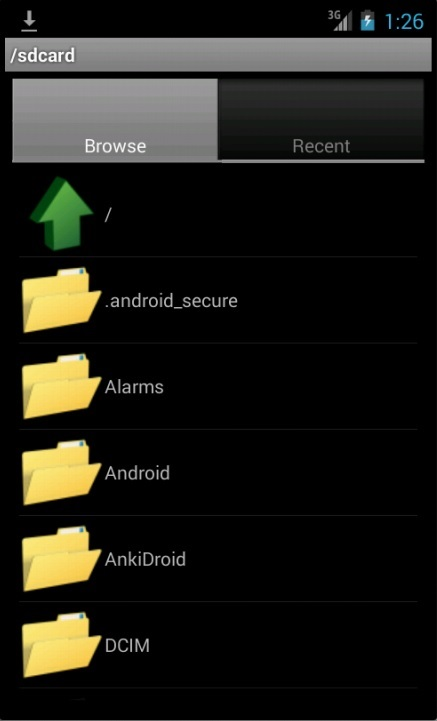
\includegraphics[width=0.225\columnwidth]{figures/bug9/bug9_shot1.jpg}
}
\hfill
\subfloat[Selecting the Recent tab.]{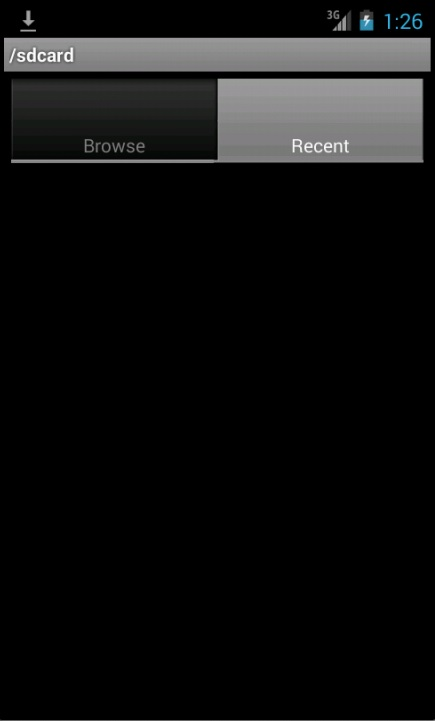
\includegraphics[width=0.225\columnwidth]{figures/bug9/bug9_shot2.jpg}
}
\hfill
\subfloat[Tab selection cleared after two rotations.]{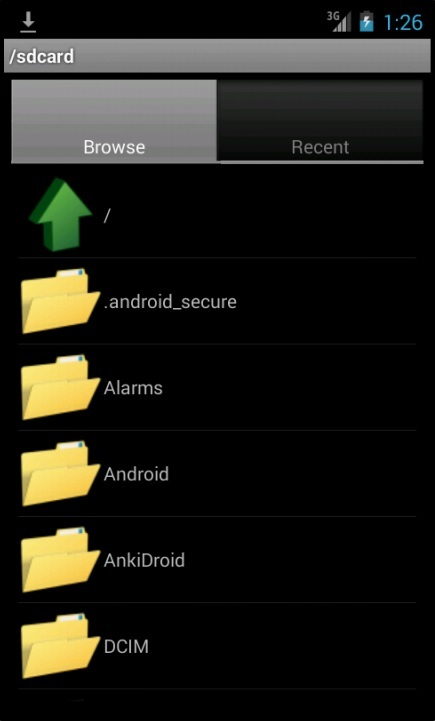
\includegraphics[width=0.225\columnwidth]{figures/bug9/bug9_shot3.jpg}
}
\caption{Rotation Bug in VuDroid.}
\label{fig:bug9}
\end{minipage}
\end{figure*}

\indent{\bf Rotation bug in Nexes Manager}: If there is an empty folder which has no permission (read, write, etc.), rotating the device makes the folder icon disappear (Figure~\ref{fig:bug10}). We reported this bug as issue 9 to Nexes Manager.
\begin{figure*}[!t]
\centering
\begin{minipage}{.5\columnwidth}
%0.36=0.18/0.5
\subfloat[The ``vendor'' folder is empty and has no permission.]{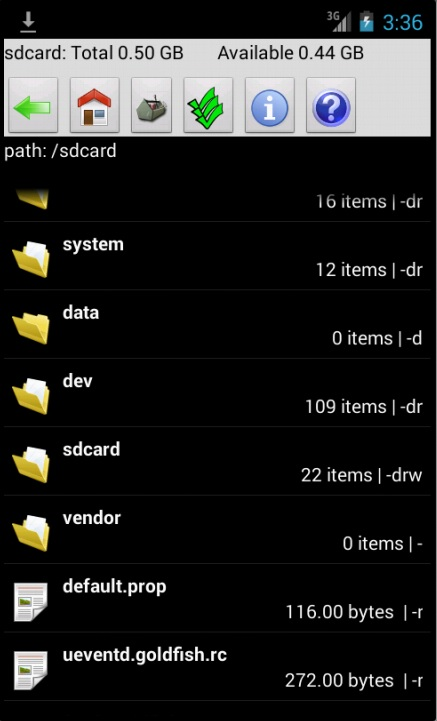
\includegraphics[width=0.36\columnwidth]{figures/bug10/bug10_shot1.jpg}
}
\hfill
\subfloat[The icon beside ``vendor'' disappears after two rotations.]{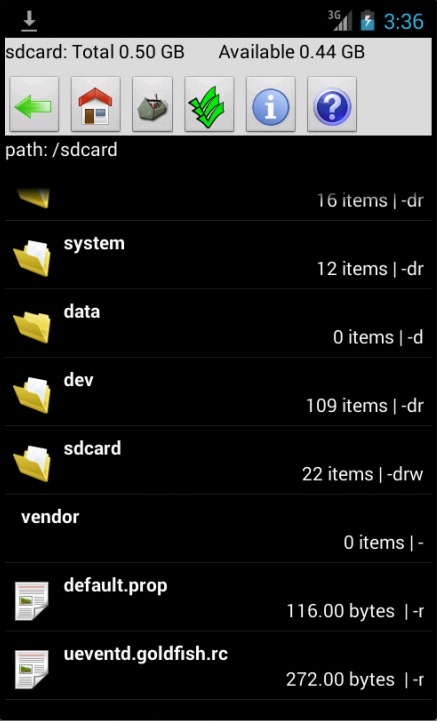
\includegraphics[width=0.36\columnwidth]{figures/bug10/bug10_shot2.jpg}
}
\caption{Rotation Bug in Nexes Manager.}
\label{fig:bug10}
\end{minipage}
\end{figure*}

\indent{\bf Back button bug in Kitchen Timer}: Going to sub-menus and coming back using the hardware Back makes buttons go out of focus. Figure~\ref{fig:bug23} shows how the plus ($+$) button is in focus, but it goes out of focus if the user navigates to the info sub-menu and then comes back using the hardware Back button. We reported this bug as issue 168 to Kitchen Timer.

\begin{figure*}[!t]
\centering
\subfloat[The $+$ button in focus.]{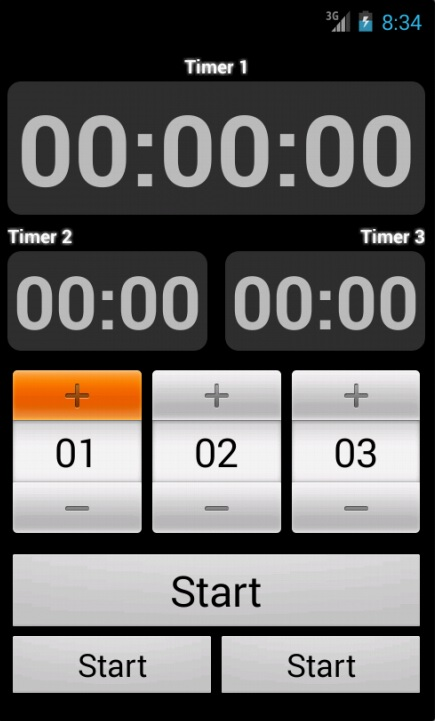
\includegraphics[width=0.18\columnwidth]{figures/bug23/bug23_shot1.jpg}
}
\hfill
\subfloat[Navigating to Menu.]{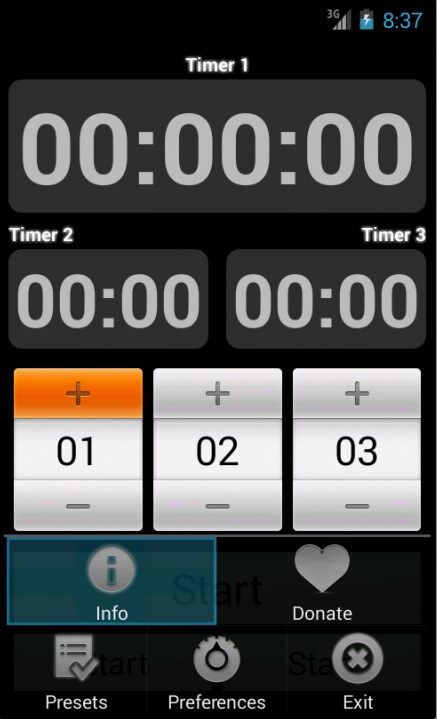
\includegraphics[width=0.18\columnwidth]{figures/bug23/bug23_shot2.jpg}
}
\hfill
\subfloat[Navigating to Menu/Info.]{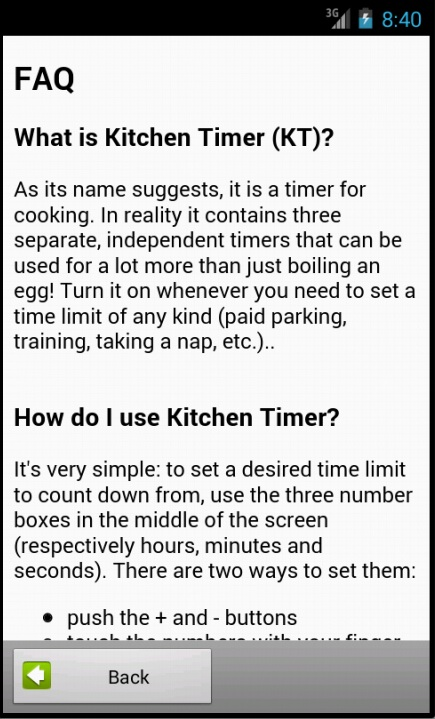
\includegraphics[width=0.18\columnwidth]{figures/bug23/bug23_shot3.jpg}
}
\hfill
\subfloat[Using the hardware Back button. $+$ goes out of focus.]{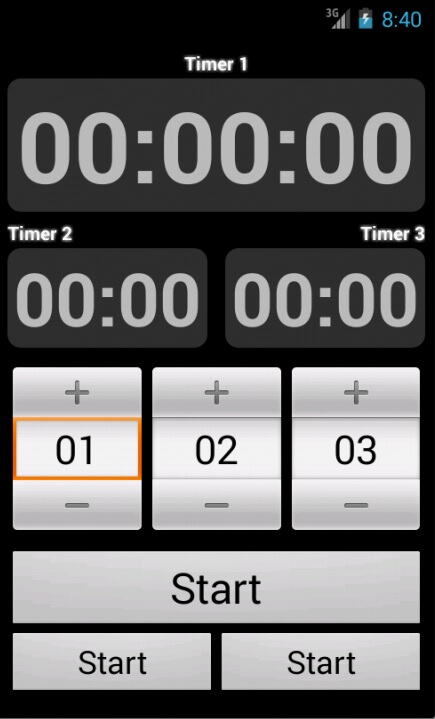
\includegraphics[width=0.18\columnwidth]{figures/bug23/bug23_shot4.jpg}
}
\caption{Back Button Bug in Kitchen Timer.}
\label{fig:bug23}
\end{figure*}

Besides the two bugs that we found already reported in the bug repositories of the corresponding apps, mentioned above as issue 7 of VuDroid and issue 161 of K9Mail, we found another pausing and resuming bug in K9Mail that was independently fixed in version 4.511. All the other \NumBugs{} bugs that \tool{} found were new.
We reported these to the respective developers (e.g., issue 121 of VuDroid, issue 5927 of K9Mail, in addition to the issues listed above) and are awaiting confirmation of the bugs from them. 
%However, we have not yet heard back from developers regarding the reports. 

\tool{} reported a total of $9$ distinct false positives. However, $4$ of these false positives were because of an inconsistency in the Android testing instrumentation, which caused it to act differently when paused programmatically (by tests) or through the emulator GUI (when manually confirming bugs). 

Another $2$ false positives were because of time sensitivity of some app states. For instance, when a timer is running in Kitchen Timer, rotation changes timer values, not because there is a bug, but rather because the state of a running timer changes with time (Figure~\ref{fig:fp6}). Such time sensitivity is usually abstracted out from the app's GUI model to achieve conciseness. 

\begin{figure*}[!t]
\centering
\begin{minipage}{.6\columnwidth}
%0.3=0.18/0.6
\subfloat[A running timer.]{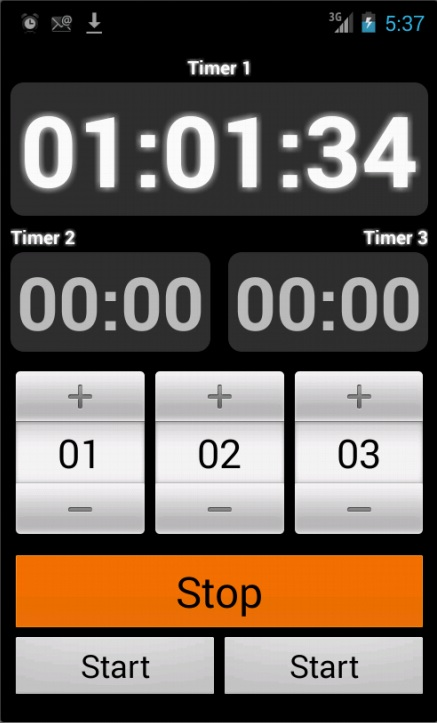
\includegraphics[width=0.3\columnwidth]{figures/fp6/fp6_shot1.jpg}
}
\hfill
\subfloat[After two rotations. A running timer changes with time.]{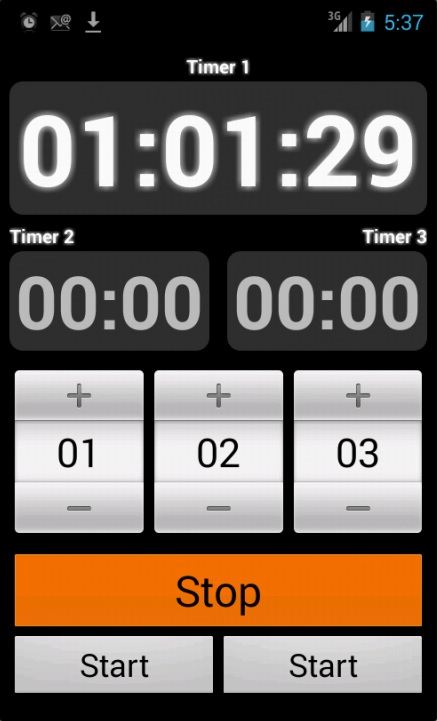
\includegraphics[width=0.3\columnwidth]{figures/fp6/fp6_shot2.jpg}
}
\caption{Time Sensitivity False Positive in Kitchen Timer.}
\label{fig:fp6}
\end{minipage}
\end{figure*}

Another $2$ false positives manifested because if the app GUI provides a visual back button on the screen, hitting this visual button and then the hardware Back button does not take the app to the original state. For example, the green arrow on the top left corner of Nexes Manager takes the app to the parent folder. However, the hardware Back button does not undo the effect of this action to take the app back to the child folder.  The remaining $1$ false positive could be considered a bug, depending on the intent of the app designer.

\begin{figure*}[!t]
\centering
\begin{minipage}{.8\columnwidth}
%0.225=0.18/0.8
\subfloat[Initial folder.]{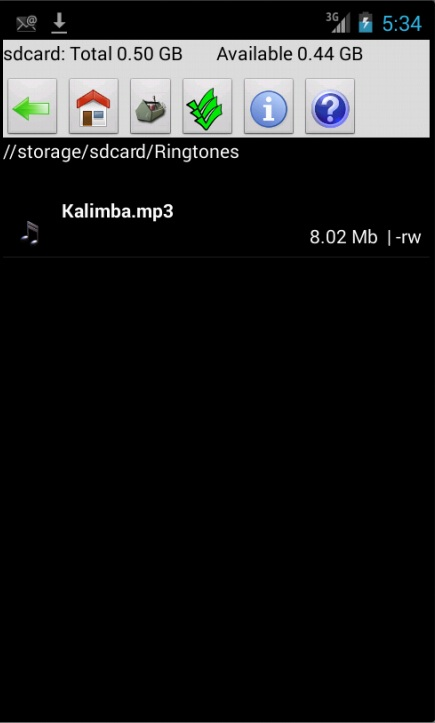
\includegraphics[width=0.225\columnwidth]{figures/fp1/fp1_shot1.jpg}
}
\hfill
\subfloat[The green arrow takes the app to the parent folder.]{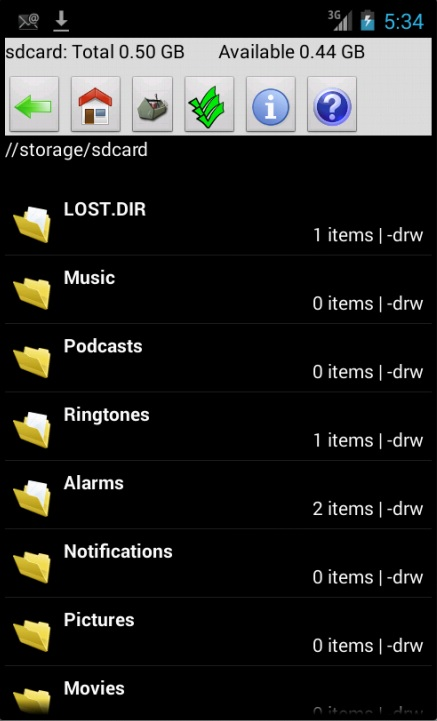
\includegraphics[width=0.225\columnwidth]{figures/fp1/fp1_shot2.jpg}
}
\hfill
\subfloat[Back does not undo the effect of the green arrow.]{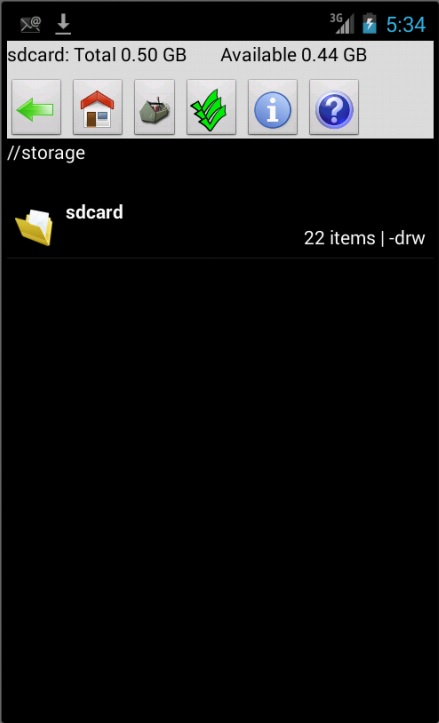
\includegraphics[width=0.225\columnwidth]{figures/fp1/fp1_shot3.jpg}
}
\caption{Back Button False Positive in Nexes Manager.}
\label{fig:fp1}
\end{minipage}
\end{figure*}



\subsection{RQ 3: Compactness of Generated Test Suites}
We compared our test generation algorithm to a baseline DFS, in generating test cases that cover all golden edges. For the set of implemented features (rotation, killing and restarting, pausing and resuming, and Back button) we measured the compactness of generated test suites in terms of the number of tests and the cost of the test suite when generated by each of the following algorithms:
%\begin{enumerate}
%\item 
(1) Our basic algorithm;
%\item 
(2) Our algorithm plus the truncation optimization, which truncates test cases after the last golden edge and ignores test cases that do not cover any golden edge;
%\item 
(3) Our algorithm plus the prioritization optimization, which prioritizes golden edges while traversing the model;
%\item 
(4) Our algorithm plus both truncation and prioritization optimizations; and
%\item 
(5) A DFS algorithm starting at the root.
%\end{enumerate}

Table~\ref{table:algoEffectiveness} shows the experimental results. The cost function is calculated with both $\alpha$ and $\beta$ set to 1. As this table shows, our algorithm shows a clear improvement over DFS, in terms of the number of tests as well as the cost of executing test suites. Furthermore, truncation and prioritization improve the results when applied separately (except for Kitchen Timer, for which truncation does not improve the number of tests or cost). In some cases (Notepad, Nexes Manager, and VuDroid), truncation yields better results compared to prioritization, while in the other cases prioritization is more effective. Fortunately, the optimizations are compatible and combinable and using both of them produces even better results for all of the studied apps.

\begin{table}[t!]
\vspace*{-3ex}
\centering
\caption{Compactness of Generated Test Suites.}
\label{table:algoEffectiveness}
{
\begin{tabular}{@{}lr@{}rrr@{}rrr@{}rrr@{}rrr@{}rr@{}}
\toprule
&&\multicolumn{11}{c}{\bf{Our Algorithm}}
&&\multicolumn{2}{c}{\bf{DFS}}\\
&&\multicolumn{2}{c}{\bf{Basic}}
&&\multicolumn{2}{c}{\bf{+ Trunc.}}
&&\multicolumn{2}{c}{\bf{+ Prior.}}
&&\multicolumn{2}{c}{\bf{+ Both}}
\\
\cmidrule{3-4}
\cmidrule{6-7}
\cmidrule{9-10}
\cmidrule{12-13}
\cmidrule{15-16}
\bf{Application}&&\begin{sideways}\bf{\#Tests}\end{sideways}&\begin{sideways}\bf{Cost}\end{sideways}&&\begin{sideways}\bf{\#Tests}\end{sideways}&\begin{sideways}\bf{Cost}\end{sideways}&&\begin{sideways}\bf{\#Tests}\end{sideways}&\begin{sideways}\bf{Cost}\end{sideways}&&\begin{sideways}\bf{\#Tests}\end{sideways}&\begin{sideways}\bf{Cost}\end{sideways}&&\begin{sideways}\bf{\#Tests}\end{sideways}&\begin{sideways}\bf{Cost}\end{sideways}\\
\midrule
\textit{Notepad}&&15&73&&11&59&&12&65&&8&44&&35&114\\
\textit{OpenSudoku}&&13&85&&10&67&&9&67&&7&51&&30&138\\
\textit{Nexes Manager}&&38&200&&24&149&&26&174&&15&127&&97&354\\
\midrule
\textit{VuDroid}&&8&41&&7&38&&7&40&&6&36&&17&57\\
\textit{Kitchen Timer}&&14&113&&14&113&&11&105&&8&75&&70&310\\
\textit{K9Mail}&&30&228&&25&196&&21&187&&16&148&&76&490\\
\bottomrule
\end{tabular}
}
\end{table}


{\bf Threats to Validity}: To minimize threats to internal validity, we automated the entire test generation and execution process and manually identified real bugs from false positives. To address external validity, we experimented with 7 previously studied apps and set forth a criterion to choose 6 other popular apps from open source repositories as discussed in Section~\ref{study}. With respect to construct validity, we strictly followed our traversal algorithm and oracle generation techniques, used well-known frameworks Robotium and JUnit, and manually investigated generated tests for some of the apps. 
One limitation of this work is synthesizing universally applicable oracles, which gives rise to false positives.
General purpose oracles are often either too weak to detect bugs or generate too many false positives. We are mitigating that short-coming by using domain specific knowledge. 


\section{Related Work}
\label{relatedwork}

%% The oracle problem in software testing: specialized oracles and automatic oracles
Our work attempts to address the classic oracle
problem~\cite{Oracle:Howden78,Weyuker80}, in the context of mobile
apps. In practice, test oracles are typically specified manually,
often at the expense of substantial time and effort. There is a rich
body of work that aims to alleviate this long-standing problem by
automatically generating oracles. Software specification mining or
model inference techniques are often used for this purpose. A
comprehensive survey of API property inference techniques by Robillard
et al. describes many of these
techniques~\cite{robillard13tse}. Automated oracle generation
techniques usually generate general purpose oracles for functional
testing; they are not specific to any platform or class of software
applications or any aspects of software behavior. However, a recent
empirical study by Nguyen et al. on the cost and effectiveness of
automated oracles concludes that their false positive rate is often
prohibitively high for practical use~\cite{Nguyen:2013}.

%% Our work: Specialized oracles
Our proposed technique does not automatically generate general purpose
oracles but rather falls into a related body of work that uses
manually created oracles based on domain specific knowledge, that are
appropriately \textit{instantiated} during testing and used to test
very specific, sometimes non-functional, aspects of software
behavior. For example, the \textsc{Toddler} tool uses a hand-crafted
oracle that detects repetitive memory access patterns in loops to
identify performance bugs in software~\cite{toddler:ICSE2013}.  Our
previous work used differential testing~\cite{McKeeman1998} for oracle
automation in the context of testing web browser
implementations~\cite{ZaeemKhurshid2012} as well as detecting
%the \textsc{X-pert} tool detects 
cross-browser errors in web applications~\cite{xpert:ICSE2013}, \ie
discrepancies in web application behavior across different web
browsers, using test oracles specifically designed for these
domain-specific applications of differential testing.
%a test oracle specifically designed for this aspect of differential
%testing of web applications.
Our work in this paper
exploits characteristics of mobile apps and the mobile platform to
design oracles for testing an important class of user-interface
features of mobile apps.  Hu et al. also employ a specialized oracle
for testing Android mobile apps, which implements and checks the
Activity life-cycle
specification\footnote{\url{http://developer.android.com/training/basics/activity-lifecycle/index.html}}
for Android apps~\cite{Hu:2011:AST}.  However, this is one single
oracle, whereas our approach proposes an extensible framework that
spans a whole class of properties -- user-interaction features.

%% Automated test sequence generation for mobile apps
There is a growing body of research focused on automated testing of mobile applications. The proposed techniques span the complete gamut of technologies from random testing~\cite{Hu:2011:AST,Dynodroid:2013}, to symbolic-execution-based test-case generation~\cite{AnandFSE2012, MirzaeiJPF2012}, model-based testing, combinatorial testing, and combinations thereof~\cite{Nguyen:2012:ISSTA, collider2013}. However, the emphasis here is on generating test sequences to maximize code coverage, for the purpose of functional testing. The oracle problem is not directly addressed in these papers. It is implicit that the oracles would either be manually specified or use the simple oracle corresponding to catastrophic failure when the application crashes, hangs or otherwise throws an exception. By contrast, the focus of our approach is precisely to address the oracle problem, for a class of non-functional and platform-specific features of mobile apps. 

Our approach to test sequence generation falls under the broad area of model-based testing. The model may be manually specified or automatically extracted from the application under test. In fact there is a rich and active body of work on reverse-engineering such models from the user-interface of GUI applications~\cite{MemonWCRE2003}, web applications~\cite{Mesbah:2012:TWEB}, and more recently, mobile applications~\cite{AmalfitanoASE2012, Joorabchi:2012:WCRE, YangFASE2013}. However, our approach is independent of the method used to produce the model and is therefore orthogonal to these techniques.

The aim of model-based test sequence generation is to extract a suite
of concrete test cases based on the behavior represented in the
model. Most techniques in this category do this by heuristically
solving some variant of the NP-Hard \textit{minimum path cover
  problem}~\cite{PathCover:NtafosH79}, typically guided by some
supporting analysis and test suite sufficiency criteria. Memon et
al. propose several test adequacy criteria for GUI testing based on
coverage of events and event-sequences in the GUI
model~\cite{memon2001coverage}. Arlt et al. use a lightweight static
analysis to compute data dependencies between event-handlers of a GUI
application and use that to guide the choice of test sequences from
the GUI model~\cite{Arlt:2012:ISSRE}. Ganov et al., on the other hand,
focus on the problem of generating suitable values for the input
parameters of abstract test sequences extracted from a GUI model and
employ symbolic execution to compute these parameter
values~\cite{Ganov:2009:ICFEM}. Nguyen et al.  address the same
problem by using combinatorial testing techniques to embed
user-specified data values into abstract test
sequences~\cite{Nguyen:2012:ISSTA}. The aim of all the above
techniques is functional testing of the application and, more
specifically, to extract test cases which maximize coverage of the
application code. By contrast, our test sequence generation is
intended to exhaustively exercise a set of platform-specific
user-interaction features. This leads to different test targets,
cost-functions and ultimately a different set of model traversal
algorithms than those by pure functional testing approaches.
%\remark{Should we mention that we target errors of omission while code-coverage based approaches do not?}
%Our coverage criteria bears similarities with using states of a finite state machine~\cite{shehady1997method} or transitions between them~\cite{belli2001finite} as coverage criteria. Our work, however, is different in that we aim to cover transitions that are originally \emph{absent} from the GUI model, since, as discussed in Section~\ref{framework}, user-interaction features are usually excluded from such models to curb state space explosion.

 

%This paper draws from the following broad areas of research.
%\begin{itemize}
%	\item \textbf{Model Generation}: GUITAR~\cite{MemonWCRE2003}, Crawljax~\cite{Mesbah:2012:TWEB}, AndroidRipper~\cite{AmalfitanoASE2012}, iOSCrawler~\cite{Joorabchi:2012:WCRE}, ORBIT~\cite{YangFASE2013}.
%	\item \textbf{Model-based Test Generation}: Selection of test sequences based on a model: \cite{Arlt:2012:ISSRE}, \cite{Nguyen:2012:ISSTA}, \cite{Ganov:2009:ICFEM}, \cite{Takala:2011}.
%	\item \textbf{Testing of Mobile Software}: Using random testing~\cite{Hu:2011:AST}, symbolic execution~\cite{AnandFSE2012}, \cite{MirzaeiJPF2012}.
%	\item \textbf{Oracles for Software Testing}: First introduced in \cite{Oracle:Howden78} and developed in \cite{Weyuker80}. Different methods of constructing oracles: from program documentation~\cite{Peters:ISSTA94}, from method post-conditions~\cite{postCondOracle:Meyer09} or using statistical methods~\cite{StatOracle:Mayer04}.  
%\end{itemize}








\section{Conclusion}
\label{conclusion}

In this paper we presented a novel approach for automatically generating test cases, complete with test oracles, for mobile apps. It was motivated by a comprehensive study that we conducted of real defects in mobile apps. Through this study we identified a class of features called user-interaction features, which were implicated in a significant fraction of bugs and for which oracles could be constructed, in an application agnostic manner, based on our common understanding of how apps behave.  Our approach, as embodied by our tool \tool, includes an extensible framework that supports such domain specific, yet application agnostic, test oracles, and automatically generates a compact suite of test sequences,
including test oracles, to comprehensively test the user-interaction features of a given mobile app. Our initial experimental evaluation of \tool\ on $\NumApps$ open-source Android apps was quite promising: \tool{} found a total of $\NumBugs$ bugs, a few of them particularly serious, using a 
total of $\NumTests$ tests for these $\NumApps$ apps. 
For future work we would like to augment the set of oracles currently supported by \tool, evaluate it more extensively on a larger set of apps, and explore the possibility of extending our basic oracle generation approach beyond the set of user-interaction features reported in this work.





% An example of a floating figure using the graphicx package.
% Note that \label must occur AFTER (or within) \caption.
% For figures, \caption should occur after the \includegraphics.
% Note that IEEEtran v1.7 and later has special internal code that
% is designed to preserve the operation of \label within \caption
% even when the captionsoff option is in effect. However, because
% of issues like this, it may be the safest practice to put all your
% \label just after \caption rather than within \caption{}.
%
% Reminder: the "draftcls" or "draftclsnofoot", not "draft", class
% option should be used if it is desired that the figures are to be
% displayed while in draft mode.
%
%\begin{figure}[!t]
%\centering
%\includegraphics[width=2.5in]{myfigure}
% where an .eps filename suffix will be assumed under latex,
% and a .pdf suffix will be assumed for pdflatex; or what has been declared
% via \DeclareGraphicsExtensions.
%\caption{Simulation Results}
%\label{fig_sim}
%\end{figure}

% Note that IEEE typically puts floats only at the top, even when this
% results in a large percentage of a column being occupied by floats.


% An example of a double column floating figure using two subfigures.
% (The subfig.sty package must be loaded for this to work.)
% The subfigure \label commands are set within each subfloat command, the
% \label for the overall figure must come after \caption.
% \hfil must be used as a separator to get equal spacing.
% The subfigure.sty package works much the same way, except \subfigure is
% used instead of \subfloat.
%
%\begin{figure*}[!t]
%\centerline{\subfloat[Case I]\includegraphics[width=2.5in]{subfigcase1}%
%\label{fig_first_case}}
%\hfil
%\subfloat[Case II]{\includegraphics[width=2.5in]{subfigcase2}%
%\label{fig_second_case}}}
%\caption{Simulation results}
%\label{fig_sim}
%\end{figure*}
%
% Note that often IEEE papers with subfigures do not employ subfigure
% captions (using the optional argument to \subfloat), but instead will
% reference/describe all of them (a), (b), etc., within the main caption.


% An example of a floating table. Note that, for IEEE style tables, the
% \caption command should come BEFORE the table. Table text will default to
% \footnotesize as IEEE normally uses this smaller font for tables.
% The \label must come after \caption as always.
%
%\begin{table}[!t]
%% increase table row spacing, adjust to taste
%\renewcommand{\arraystretch}{1.3}
% if using array.sty, it might be a good idea to tweak the value of
% \extrarowheight as needed to properly center the text within the cells
%\caption{An Example of a Table}
%\label{table_example}
%\centering
%% Some packages, such as MDW tools, offer better commands for making tables
%% than the plain LaTeX2e tabular which is used here.
%\begin{tabular}{|c||c|}
%\hline
%One & Two\\
%\hline
%Three & Four\\
%\hline
%\end{tabular}
%\end{table}


% Note that IEEE does not put floats in the very first column - or typically
% anywhere on the first page for that matter. Also, in-text middle ("here")
% positioning is not used. Most IEEE journals/conferences use top floats
% exclusively. Note that, LaTeX2e, unlike IEEE journals/conferences, places
% footnotes above bottom floats. This can be corrected via the \fnbelowfloat
% command of the stfloats package.

%\vspace*{-2ex}
\section*{Acknowledgment}
%\vspace*{-1ex}
We thank Guowei Yang for detailed discussions and comments on this work. This work was funded in part by the Fujitsu Labs of America (SRA No. UTA12-001194) and the National Science Foundation (NSF Grant Nos. CCF-0845628 and CNS-1239498).
\vspace*{-2ex}

% trigger a \newpage just before the given reference
% number - used to balance the columns on the last page
% adjust value as needed - may need to be readjusted if
% the document is modified later
%\IEEEtriggeratref{8}
% The "triggered" command can be changed if desired:
%\IEEEtriggercmd{\enlargethispage{-5in}}

% references section

% can use a bibliography generated by BibTeX as a .bbl file
% BibTeX documentation can be easily obtained at:
% http://www.ctan.org/tex-archive/biblio/bibtex/contrib/doc/
% The IEEEtran BibTeX style support page is at:
% http://www.michaelshell.org/tex/ieeetran/bibtex/
%\bibliographystyle{IEEEtran}
% argument is your BibTeX string definitions and bibliography database(s)
%\bibliography{IEEEabrv,../bib/paper}
%
% <OR> manually copy in the resultant .bbl file
% set second argument of \begin to the number of references
% (used to reserve space for the reference number labels box)
%\begin{thebibliography}{1}
%
%\bibitem{IEEEhowto:kopka}
%H.~Kopka and P.~W. Daly, \emph{A Guide to \LaTeX}, 3rd~ed.\hskip 1em plus
%  0.5em minus 0.4em\relax Harlow, England: Addison-Wesley, 1999.
%
%\end{thebibliography}


\vspace*{-2ex}
\bibliographystyle{plain}
\bibliography{paper}

% that's all folks
\end{document}


